%%%%%%%%%%%%%%%%%%% vorlage.tex %%%%%%%%%%%%%%%%%%%%%%%%%%%%%
%
% LaTeX-Vorlage zur Erstellung von Projekt-Dokumentationen
% im Fachbereich Informatik der Hochschule Trier
%
% Basis: Vorlage svmono des Springer Verlags
%
%%%%%%%%%%%%%%%%%%%%%%%%%%%%%%%%%%%%%%%%%%%%%%%%%%%%%%%%%%%%%

\documentclass[envcountsame,envcountchap, deutsch]{i-studis}

\usepackage{makeidx}         	% Index
\usepackage{multicol}        	% Zweispaltiger Index
\usepackage{listings}
%\usepackage[bottom]{footmisc}	% Erzeugung von Fu�noten

%%-----------------------------------------------------
%\newif\ifpdf
%\ifx\pdfoutput\undefined
%\pdffalse
%\else
%\pdfoutput=1
%\pdftrue
%\fi
%%--------------------------------------------------------
%\ifpdf
\usepackage[pdftex]{graphicx}
\usepackage{epstopdf}
\usepackage[pdftex,plainpages=false]{hyperref}
\usepackage{amssymb}
%\else
%\usepackage{graphicx}
%\usepackage[plainpages=false]{hyperref}
%\fi

%%-----------------------------------------------------
\usepackage{color}				% Farbverwaltung
%\usepackage{ngerman} 			% Neue deutsche Rechtsschreibung
\usepackage[english, ngerman]{babel}
\usepackage[latin1]{inputenc} 	% Erm�glicht Umlaute-Darstellung
%\usepackage[utf8]{inputenc}  	% Erm�glicht Umlaute-Darstellung unter Linux (je nach verwendetem Format)

%-----------------------------------------------------
\usepackage{listings} 			% Code-Darstellung
\lstset
{
	basicstyle=\scriptsize, 	% print whole listing small
	keywordstyle=\color{blue}\bfseries,
								% underlined bold black keywords
	identifierstyle=, 			% nothing happens
	commentstyle=\color{red}, 	% white comments
	stringstyle=\ttfamily, 		% typewriter type for strings
	showstringspaces=false, 	% no special string spaces
	framexleftmargin=7mm, 
	tabsize=3,
	showtabs=false,
	frame=single, 
	rulesepcolor=\color{blue},
	numbers=left,
	linewidth=146mm,
	xleftmargin=8mm
}
\usepackage{textcomp} 			% Celsius-Darstellung
\usepackage{amssymb,amsfonts,amstext,amsmath}	% Mathematische Symbole
\usepackage[german, ruled, vlined]{algorithm2e}
\usepackage[a4paper]{geometry} % Andere Formatierung
\usepackage{bibgerm}
\usepackage{array}
\hyphenation{Ele-men-tar-ob-jek-te  ab-ge-tas-tet Aus-wer-tung House-holder-Matrix Le-ast-Squa-res-Al-go-ri-th-men} 		% Weitere Silbentrennung bei Bedarf angeben
\setlength{\textheight}{1.1\textheight}
\pagestyle{myheadings} 			% Erzeugt selbstdefinierte Kopfzeile
\makeindex 						% Index-Erstellung


%--------------------------------------------------------------------------
\begin{document}
%------------------------- Titelblatt -------------------------------------
\title{Konzeption und Realisierung eines Systems zur Informationssuche in einem Dokumentenarchiv basierend auf Textinhalt und Metadaten. }
\subtitle{Conception and Realization of an Information Retrival System for a Document Archive based on Text Content and Metadata}
%---- Die Art der Dokumentation kann hier ausgew�hlt werden---------------
%\project{Bachelor-Projektarbeit}
\project{Bachelor-Abschlussarbeit}
%\project{Master-Projektstudium}
%\project{Master-Abschlussarbeit}
%\project{Seminar zur Vorlesung ...}
%\project{Hausarbeit zur Vorlesung ...}
%--------------------------------------------------------------------------
\supervisor{Prof. Dr. Karl Hans Bl�sius} 		% Betreuer der Arbeit
\author{Annika Kremer} 							% Autor der Arbeit
\address{Trier,} 							% Im Zusammenhang mit dem Datum wird hinter dem Ort ein Komma angegeben
\submitdate{Abgabedatum} 				% Abgabedatum
%\begingroup
%  \renewcommand{\thepage}{title}
%  \mytitlepage
%  \newpage
%\endgroup
\begingroup
  \renewcommand{\thepage}{Titel}
  \mytitlepage
  \newpage
\endgroup
%--------------------------------------------------------------------------
\frontmatter 
%--------------------------------------------------------------------------
%\preface

Ein Vorwort ist nicht unbedingt n�tig. Falls Sie ein Vorwort schreiben, so ist dies der Platz, um z.B. die Firma vorzustellen, in der diese Arbeit entstanden ist, oder einigen Leuten zu danken, die in irgendeiner Form positiv zur Entstehung dieser Arbeit beigetragen haben. Auf keinen Fall sollten Sie im Vorwort die Aufgabenstellung n�her erl�utern oder vertieft auf technische Sachverhalte eingehen.				% Vorwort (optional)
\kurzfassung

%% deutsch
\paragraph*{}
%In der Kurzfassung soll in kurzer und pr�gnanter Weise der wesentliche Inhalt der Arbeit beschrieben werden. Dazu z�hlen vor allem eine kurze Aufgabenbeschreibung, der L�sungsansatz sowie die wesentlichen Ergebnisse der Arbeit. Ein h�ufiger Fehler f�r die Kurzfassung ist, dass lediglich die Aufgabenbeschreibung (d.h. das Problem) in Kurzform vorgelegt wird. Die Kurzfassung soll aber die gesamte Arbeit widerspiegeln. Deshalb sind vor allem die erzielten Ergebnisse darzustellen. Die Kurzfassung soll etwa eine halbe bis ganze DIN-A4-Seite umfassen.

%Hinweis: Schreiben Sie die Kurzfassung am Ende der Arbeit, denn eventuell ist Ihnen beim Schreiben erst vollends klar geworden, was das Wesentliche der Arbeit ist bzw. welche Schwerpunkte Sie bei der Arbeit gesetzt haben. Andernfalls laufen Sie Gefahr, dass die Kurzfassung nicht zum Rest der Arbeit passt.



Diese Arbeit befasst sich mit der Konzeption und Realisierung eines Information-Retrieval-Systems, welches ein Archiv mit semistrukturierten Dokumenten, die sowohl Freitext als auch Metadaten enthalten, effizient nach vom Nutzer festgelegten und logisch verkn�pfbaren Kriterien durchsucht. Ziel der Implementierung ist es, dem Nutzer nach Abschluss des Suchvorgangs zu seinem Informationsbed�rfnis passende Dokumente zur�ckzuliefern und diese auf eine �bersichtliche Weise zu pr�sentieren. \\
Zun�chst wird die Problemstellung im Detail erl�utert, damit der Leser eine genaue Vorstellung �ber die Anforderungen, welche die Implementierung erf�llen soll, bekommt. Anschlie�end wird Information Retrieval im Allgemeinen vorgestellt, um einen �berblick �ber die Thematik zu geben. 
Es folgt eine Vorstellung der beiden klassischen Information Retrieval Modelle boolesches Retrieval und Vektorraummodell inklusive Erl�uterung der Funktionsweisen. Anschlie�end wird beschrieben, wie sich solche Modelle in Hinsicht auf deren Qualit�t bewerten und vergleichen lassen.\\
Nach dem Vermitteln der notwendigen theoretischen Kenntnisse beschreibt der Implementierungsteil, auf welche Weise und in welchen Bereichen die beiden Verfahren f�r die Implementierung zum Einsatz kamen und inwieweit eine Modifizierung zur Anpassung auf die vorliegende Problemstellung erfolgte. 
Neben der internen Funktionsweise wird auch die Benutzung der Oberfl�che erl�utert, um den Anwender mit der Bedienung des Systems vertraut zu machen.  \\
Es folgt eine Zusammenfassung der Arbeit mit abschlie�ender Bewertung der Ergebnisse sowie ein Ausblick auf zuk�nftige Verbesserungsm�glichkeiten.
\newpage
\paragraph*{}
This paper discusses the conception and realization of an information retrieval system that searches efficiently in semistructured data containing free text and metadata. The  search criteria for this system are determined by the user and can be freely connected with boolean operators. The aim of the implementation is to retrieve documents satysfying the user's information need and to present the results clearly.\\
First the problem is discussed in detail to give the reader a precise idea of the requirements which the implementation has to fit. Afterwards, information retrieval in general is presented to give an overview on the topic.
The chapter about information retrieval is followed by a presentation of two classical information retrieval model including their functionality called boolean retrieval and vectorspace model. Afterwards, it is discussed how the quality of such systems can be estimated and compared. \\
After having provided the necessary theory, the paper continues with the implementation part, which explains which models were used in which way and if they have been modified in any way to fit this problem. 
Aside from the intern functionality, the reader learns about how to operate with the system via the given user interface. \\
The paper concludes with a summary including a final result evaluation and a presentation of future prospects for system improvements.




 			% Kurzfassung Deutsch/English
\tableofcontents 						% Inhaltsverzeichnis
\listoffigures 							% Abbildungsverzeichnis (optional)
\listoftables 							% Tabellenverzeichnis (optional)
%--------------------------------------------------------------------------
\mainmatter                        		% Hauptteil (ab hier arab. Seitenzahlen)
%--------------------------------------------------------------------------
% Die Kapitel werden in separaten .tex-Dateien abgelegt und hier eingebunden.
\chapter{Einleitung und Problemstellung}

\section{Einleitung}

Wer kennt es nicht: Tagt�glich treffen neue E-Mails ein, sodass das Postfach sich immer weiter f�llt. \\
Schnell ist es passiert, dass die Menge an Nachrichten un�bersichtlich gro� wird, was zu einem ernsthaften Problem wird, sobald man etwas bestimmtes darin wiederfinden m�chte. \\
Die ben�tigte Mail war wichtig, weil sie eine bestimmte Kontaktadresse enthielt, aber wie war nochmal der Absender? L�ngst vergessen. Das genaue Datum? Leider ist nur noch der Monat bekannt. Wer jetzt manuell suchen muss, ist an dieser Stelle verloren. \\
Abhilfe schafft ein Information Retrieval System, mit dem man bestimmte Suchkriterien eingeben und beliebig miteinander kombinieren kann. \\
 So bekommt der Nutzer genau die Nachrichten pr�sentiert, die sein Informationsbed�rfnis am ehesten bedienen, und  braucht sich nicht erst durch hunderte von Mails durchzuarbeiten. In diesem Fall k�nnte die Person beispielsweise im Freitext nach dem Wort \glqq Kontaktadresse\grqq{} suchen und weitere Kriterien wie \glqq Datum = Juni \grqq{} hinzuf�gen. \\
Besonderheit ist das beliebige Verkn�pfen: Der Nutzer kann sich entscheiden, ob er nur Resultate akzeptiert, auf die Beides zutrifft, oder ob es bereits reicht, wenn eines der Kriterien erf�llt ist. Dies erlaubt eine sehr individuelle, auf den Benutzer zugeschnittene Suche. \\
Ein solches System ist nicht nur f�r das Alltagsbeispiel E-Mail-Ordner, d.h. Posteingang, Postausgang etc. wertvoll, sondern l�sst sich auch auf jede andere Art von Dokumentenarchiv, dessen Dokumente sowohl Freitext als auch Metadaten beinhalten, anwenden. 





\section{Problemstellung}

Ziel der Arbeit ist die Konzeption und Realisierung eines Systems zur Informationssuche (engl. Information Retrieval System) in einem Dokumentenarchiv, wobei die Dokumente von teilweise strukturierter Natur sind. \\
Dies bedeutet, dass sie sowohl gew�hnlichen Freitext als auch Metadaten enthalten. Der Nutzer soll spezifizieren k�nnen, in welchen Metadaten er suchen m�chte, zudem soll die Freitextsuche ausw�hlbar sein. Alle Suchanfragen sollen hierbei beliebig mit den booleschen Operatoren \textit{AND} (engl. und) sowie \textit{OR} (engl. oder) verkn�pfbar sein. \\
Hauptanwendungszweck des Systems sind E-Mail-Archive wie Posteingang und Postausgang, allerdings soll das System so flexibel sein, dass es auch auf andere teilweise strukturierte Dokumentenarchive anwendbar ist. 


\section{Teilprobleme}
Aus der Aufgabenstellung ergeben sich die im folgenden beschriebenen Teilprobleme.


\subsection{Dynamisches einlesen der Metadaten}
Die genauen Metadaten sind, da das System flexibel sein soll, vor dem Ausf�hren des Systems noch nicht bekannt. Demnach muss das IR-System die Namen der Metadaten beim Starten des Programms dynamisch einlesen und diese dem Nutzer auf der grafischen Oberfl�che anzeigen.

\subsection{Unterscheidung Metadaten und Freitext}
Damit das System die Metadaten dynamisch einlesen kann, m�ssen die folgenden Punkte erf�llt sein:
\begin{enumerate}
	\item Das System muss zwischen Metadaten und Freitext unterscheiden k�nnen.
	\item Metadaten setzen sich aus Name und Inhalt zusammen, weshalb beides erkannt und voneinander abgegrenzt werden muss. Im folgenden werden die Namen als \glqq Keywords \grqq{} bezeichnet.
	\item Der Inhalt kann unterschiedlichen Datentyps sein, z.B. String oder Liste, weshalb dieser bestimmt werden muss.
\end{enumerate}


\subsection{Metadatensuche}
Es muss erkannt werden, welche Metadaten der Nutzer ausgew�hlt hat und in genau diesen muss, unter Ber�cksichtigung des jeweiligen Datentyps der Inhalte, gesucht werden. \\
Im Gegensatz zur Freitextsuche muss zu jedem Dokument vor der Suche zun�chst gepr�ft werden, ob das entsprechende Schl�sselwort �berhaupt darin auftritt.

\subsection{Freitextsuche}
Bei der Freitextsuche ist die Wortzahl weitaus gr��er als bei der Metadatensuche. Daraus resultieren zwei Probleme:
\begin {enumerate}
\item Wie kann effizient in gro�en Wortmengen gesucht werden?
\item Wie kann die Suche bei begrenztem Speicher bew�ltigt werden?
\end{enumerate}

Zudem stellt sich die Frage nach einem geeigneten Verfahren, das bei l�ngeren Anfragen auch teilweise passende Ergebnisse liefert und messen kann, wie gut die erzielten Treffer zur Nutzeranfrage passen.


\subsection{Verkn�pfung mit UND/ODER}
Alle Anfragen sollen beliebig mit den logischen Operatoren \textit{AND}, \textit{OR} sowie \textit{NOT} verkn�pfbar sein. Dies beinhaltet die folgenden Problemstellungen:
\begin{enumerate}
\item Keywordsuche und Freitextsuche m�ssen miteinander verkn�pft werden.
\item Sind meherere Keywords ausgew�hlt, m�ssen die Teilergebnisse verkn�pft werden.
\item Stellt der Nutzer mehrere Anfragen, m�ssen die Ergebnisse der einzelnen Anfragen verkn�pft werden.
	\end{enumerate}






\subsection{Benutzeroberfl�che}
Der Nutzer ben�tigt eine verst�ndliche Benutzeroberfl�che, die es ihm erm�glicht, seine Suchanfragen beliebig zusammenzustellen. Hierzu muss die Oberfl�che folgende grundlegenden Funktionalit�ten aufweisen:
\begin{enumerate}
	\item Das Suchverzeichnis, d.h. das Dokumentenarchiv in welchem die Suche stattfindet, muss ausw�hlbar sein. 
	\item Alle im Archiv auftretenden Keywords sowie die Freitextsuche m�ssen ausw�hlbar sein.
	\item Logische Operatoren (AND,OR,NOT) zur Verkn�pfung m�ssen ausw�hlbar sein.
	\item Die Suchanfrage muss f�r den Nutzer verst�ndlich angezeigt werden.
	
	
\end{enumerate}

\chapter{Information Retrieval}
Dieses Kapitel soll dem Leser einen �berblick �ber die Bedeutung des Begriffs \glqq Information Retrieval\grqq{} vermitteln.


\section{Bedeutung}


Der aus dem Englischen stammende Begriff \glqq Information Retrieval\grqq{} l�sst sich mit \glqq Informationsr�ckgewinnung\grqq{} ins Deutsche �bersetzen (\cite{Academic:12}). Hierbei wird explizit von \textit{R�ck}gewinnung gesprochen, da keine neuen Informationen erzeugt werden, sondern auf bereits existierende zugegriffen wird. 
Bevor auf die genaue Bedeutung eingegangen wird, erfolgt zun�chst die in dieser Arbeit verwendete Definition des im Ausdruck enthaltenen Teilbegriffs \glqq Information\grqq{}. 

 
\subsection{Information}
\label{info}
Der Begriff stammt von dem lateinischen Wort \textit{informare}, was sich mit \glqq Gestalt geben\grqq{} �bersetzen l�sst und im �bertragenen Sinne \glqq jemanden durch Unterweisung bilden\grqq{} bedeutet (\cite{Claus:06}, S.314-315). \\
Dies betont den Aspekt, dass eine Information stets einen Empf�nger besitzt, welcher \glqq gebildet\grqq{} wird. Dieser kann eine Person, aber auch ein geeignetes, nach au�en wirksames System sein. 
Erst das Aufnehmen und korrekte Interpretieren durch einen Empf�nger macht aus Daten als Informationstr�gern tats�chlich Informationen. 
Die Informationen m�ssen deshalb auf eine von Menschen bzw. Systemen interpretierbare Weise dargestellt werden, beispielsweise durch alphabetische Zeichen. Zudem muss es hierf�r einen geeigneten Tr�ger, z.B. ein Textdokument, geben (\cite{Claus:06}, S.314-315). \\
Informationen lassen sich in die folgenden drei Bestandteile zerlegen (\cite{Claus:06}, S.314-315): 

\begin{itemize}
	\item \textit{Syntaktischer Teil:} Ist die Struktur der Information syntaktisch zul�ssig? Beispiel hierf�r ist die Einhaltung von Rechtschreibung und Grammatik bei Texten.
	\item \textit{Semantischer Teil:} Welche inhaltliche Bedeutung besitzt die Information? 
	\item \textit{Pragmatischer Teil:} Welchem Zweck dient sie?
\end{itemize} 


\subsection{Begriffsdefinition}
Nach dem der Teilbegriff \glqq Information\grqq{} vorgestellt wurde, wird in diesem Abschnitt auf die Bedeutung von Information Retrieval eingegangen.
Auch hier ist es problematisch, eine einheitliche Definition zu finden. Eine m�gliche Erkl�rung lautet wie folgt: \\


\begin{definition} (Information Retrieval) \\
	\label{Def}
Mit Information Retrieval, kurz IR, wird das Auffinden von in unstrukturierter Form vorliegender und ein Informationsbed�rfnis befriedigender Materialien innerhalb gro�er Sammlungen bezeichnet (\cite{Manning:08}, S.1). \\


\end{definition}
Mit unstrukturierten Materialien sind hierbei meist Dokumente in Textform gemeint, \glqq unstrukturiert\grqq{} bezeichnet jedoch allgemein alle Dokumente ohne eine klar vorgegebene, f�r einen Computer leicht zu verarbeitende Struktur. In der Praxis sind nur die wenigsten Daten vollkommen unstrukturiert, da selbst Texte einer vorgegebenen Grammatik der jeweiligen Sprache folgen. Der Begriff darf darum nicht zu streng genommen werden, vor allem da auch semistrukturierte Dokumente, die nur teilweise Freitext beinhalten, unter die Definition von Information Retrieval fallen.  Das Gegenteil stellen strukturierte Daten wie beispielsweise Datenbanken dar, die f�r einen Computer leicht zu verarbeiten sind. �blicherweise liegen die Sammlungen auf dem Computer gespeichert vor (\cite{Manning:08}, S.1-2). \\

\subsection{Unterschied zur Datenbankensuche}
Zum besseren Verst�ndnis hilft eine Abgrenzung zur Datenbanksuche, denn in Datenbanken liegen die Daten strukturiert in Form von Werttupeln bekannten Datentyps vor, was Definition \ref{Def} widerspricht.
Ein wesentliches Unterscheidungsmerkmal zwischen Information Retrieval und Datenbanksuche ist, dass bei der Datenbankensuche nicht mit vagen Anfragen umgegangen werden kann: Es kann zwar nach $(Miete < 300)$ gesucht werden, aber mit \textit{\glqq g�nstige Miete\grqq{}} w�re die Datenbank �berfordert: Wie ist g�nstig zu interpretieren? 
Ein Information-Retrieval-System kann hingegen solche Anfragen mit nicht genau definierter Bedeutung verarbeiten (\cite{Ferber:03}, S.10-11).


\section{Beispiel Websuche}
An dieser Stelle soll ein bekanntes Beispiel f�r Information Retrieval zur Veranschaulichung gegeben werden. 
Nahezu jeder benutzt im Alltag Web-Suchmaschinen.
Die Websuche stellt einen typischen Fall von Information Retrieval dar, was durch die Anwendung von Definition \ref{Def} deutlich wird: Hier sollen Freitext beinhaltende, d.h. unstrukturierte Dokumente (z.B. im HTML- oder pdf-Format) innerhalb des World Wide Webs aufgefunden werden, um das Informationsbed�rfnis des Internetnutzers zu befriedigen (\cite{Ferber:03}, S.6).
Relevante Suchergebnisse sind demnach Dokumente, welche die gesuchte Information beinhalten. Diese l�sst sich, wie in Abschnitt \ref{info} beschrieben, in drei Teile zerlegen, wobei der semantische Teil die Herausforderung f�r das Information-Retrieval-System darstellt. \\
Hierzu ein spezifisches Beispiel:
M�chte der Nutzer demn�chst seinen Urlaub in Kreta verbringen, k�nnte seine Suchanfrage \textit{\glqq Hotel g�nstig Kreta\grqq{}} lauten.
Der pragmatische Teil besteht darin, den Urlaub zu planen. Der syntaktische Teil ist ebenfalls leicht zu bestimmen: Die gesuchten Begriffe oder hierzu verwandte W�rter m�ssen in den Dokumenten auftauchen.
Als schwierig gestaltet sich hingegen der semantische Teil: Die Inhalte der Resultate m�ssen mit der urspr�nglichen Intention des Nutzers �bereinstimmen. Diese ist allerdings vage formuliert: Der Begriff \glqq g�nstig\grqq{} ist nicht n�her definiert. Nur ein Teil der Hotels, welche in der Ergebnisliste erscheinen, werden mit den Anspr�chen des Nutzers �bereinstimmen, vielleicht auch gar keine. Ein gutes Information-Retrieval-System zeichnet sich durch einen m�glichst gro�en Anteil relevanter Resultate unter allen zur�ckgelieferten Dokumenten aus. \\
H�ufig passiert es, dass zwar der syntaktische Teil erf�llt ist, d.h. die Suchbegriffe tauchen zwar im Dokument auf, allerdings stimmt der Kontext nicht mit dem Informationsbed�rfnis des Nutzers �berein. Dieses Problem tritt bei der Datenbanksuche, wo es keinerlei Interpretationsfreiraum gibt, gar nicht erst auf. 



\section{Bezug zur Problemstellung}
Dieser Abschnitt soll erkl�ren, inwiefern es sich bei der gegebenen Problemstellung um ein Information-Retrieval-Problem handelt.
Die Aufgabe besteht kurz gefasst darin, nach vom Nutzer ausgew�hlten, logisch verkn�pften Kriterien innerhalb eines Dokumentenarchivs zu suchen (siehe Abschnitt \ref{Problemstellung}). 
Damit ist die Definition \ref{Def} erf�llt, da hier Materialien innerhalb einer Sammlung, dem Dokumentenarchiv, aufgefunden werden sollen, um ein Informationsbed�rfnis zu befriedigen. \\
Dieses Bed�rfnis unterscheidet sich nat�rlich von Anfrage zu Anfrage, besteht aber allgemein gefasst darin, Dokumente wiederzufinden, z.B. eine bestimmte E-Mail. \\

\subsection{Teilweise strukturierte Daten}
Eine Besonderheit der Problemstellung ist hierbei, dass die Dokumente teilweise strukturiert sind, d.h. es liegt zwar Freitext vor, was mit Definition \ref{Def} �bereinstimmt, aber zus�tzlich sind strukturierte Metadaten vorhanden. 
Im Falle der Freitextsuche l�sst sich aufgrund der unstrukturierten Textform eindeutig von Information Retrieval sprechen, anders sieht es hingegen bei den Metadaten aus, welche die folgende Syntax und damit Struktur besitzen: \\

(Name Inhalt)\\

Es liegt dennoch ein Information-Retrieval-Problem vor, da der Begriff auch die Suche in teilweise strukturierten oder semistrukturierten Dokumenten einschlie�t (\cite{Manning:08}, S.1-2). 
Genau betrachtet sind selbst die Metadaten nicht vollkommen strukturiert: Der Datentyp des Inhalts ist offen gelassen und es gibt keinerlei Vorgaben, welche Metadaten in den Dokumenten auftreten m�ssen.  \\
In den folgenden Kapiteln wird beschrieben, auf welche Weise ein Information-Retrieval-System, das die gegebene Problemstellung l�st, konzipiert und realisiert werden kann.
 Hierzu werden zun�chst die hierf�r ben�tigten Kenntnisse �ber die beiden klassischen Information-Retrieval-Verfahren boolesches Retrieval (siehe Kapitel \ref{bool}) und Vektorraummodell (siehe Kapitel \ref{vector}) vermittelt.
 









\chapter{Grundbegriffe}
Unabh�ngig vom jeweiligen Modell gibt es einige Grundbegriffe, welche im Zusammenhang mit Information Retrieval Verfahren immer wieder auftauchen und die darum vorab vorgestellt werden sollen. 

\section{Anfrage}
Eine Anfrage (engl. query) ist das, was der Anwender in den Computer eingibt, um sein Informationsbed�rfnis zu befriedigen (\cite{Manning:08}, S.5). \\
Anfragen k�nnen je nach Information Retrieval System vollkommen unterschiedlich strukturiert sein. Wichtig ist, dass der Nutzer wei� wie er seine Anfrage stellen muss, um mehr �ber das gew�nschte Thema zu erfahren, was bei booleschen Modellen (siehe Kapitel \ref{bool}) recht komplex werden kann. \\


\section{Indexierung}
Damit Dokumente eines Archivs von Information Retrieval Modellen verarbeitet werden k�nnen, m�ssen diese in einzelne Einheiten zerlegt werden, wobei jede Einheit mit einem eindeutigen Index versehen sein muss, um hinterher mit einem schnellen Zugriff abrufbar zu sein. \\
Zudem m�ssen auch die Dokumente selbst mit einem Index versehen werden, genannt \textit{docID} (kurz f�r \textit{document identification}), um auf deren enthaltende Einheiten schnell zugreifen zu k�nnen. Dabei handelt es sich meist um einen ganzzahligen Wert (\cite{Manning:08}, S.7).\\
Dieses Vorgehen wird als Indexierung bezeichnet und ist unabdingbar, da ansonsten f�r jede Anfrage erneut �ber die gesamten Dokumentinhalte iteriert werden m�sste, was ineffizient und f�r den Nutzer unzumutbar langsam w�re (\cite{Manning:08}, S.3). \\

\subsection{Term und Vokabular}
Die indizierten Einheiten, in welche die Dokumente zerlegt werden, sind unter dem Begriff Term bekannt (\cite{Manning:08}, S.3).\\
Terme sind im h�ufigsten Fall einfach W�rter eines Textes, dies muss jedoch nicht zwangsl�ufig der Fall sein.\\
Manche Systeme reduzieren W�rter beispielsweise auf deren Stammformen, um �hnliche W�rter zu einem einzigen Term zusammenzufassen. Alternativ lassen sich W�rter neben dem Wortstamm auch auf ihre grammatikalische Grundform reduzieren. Das Reduzieren der W�rter wird allgemein als Lemmatisierung oder Stemming bezeichnet.\\ Auf diese Weise m�ssen weniger Terme verwaltet werden, was den Speicherbedarf reduziert. Au�erdem k�nnen leichter �hnliche Dokumente gefunden werden, da auch zum Suchbegriff verwandte W�rter zu einem Treffer f�hren (\cite{Ferber:03}, S.40-41). \\
 Die Menge aller unterschiedlichen Terme eines Archivs wird als Vokabular bezeichnet (\cite{Manning:08}, S.6). \\




\subsection{Stopwords}
Nicht jedes Wort wird bei der Indexierung zu einem Term: Handelt es sich um sehr h�ufig auftretende und zum Sinn des Textes wenig beitragende W�rter, wie z.B. \glqq und\grqq{} oder \glqq dann\grqq{}, k�nnen diese wegfallen, um Speicherplatz zu sparen (\cite{Ferber:03}, S.37). Au�erdem kommen durch ignorieren unwichtiger Terme weniger Dokumente infrage, was die Suche beschleunigt.\\




\chapter{Boolesches Retrieval}
\label{bool}
Dieses Kapitel stellt das klassische Information-Retrieval-Verfahren boolesches Retrieval (engl.Boolean Retrieval) vor. \\

\section{Eigenschaften des Verfahrens}
Boolesches Retrieval �berpr�ft Dokumente darauf, ob eine bestimmte Bedingung zutrifft.\\
Somit gibt es nur die Unterteilung in passende Dokumente und solche, welche die Bedingung nicht erf�llen. Eine weitere Bewertung der Ergebnisse findet nicht statt (\cite{Ferber:03}, S.33). Das fehlende Ranking der Ergebnisse ist ein h�ufiger Kritikpunkt des Verfahrens.\\
 
 
\section{Funktionsprinzip}
Boolesches Retrieval basiert auf Mengenoperationen. Deshalb werden Dokumente Mengen zugeordnet, die jeweils durch bestimmte Attribute charakterisiert sind. \\
Dokument bezeichnet die Einheit, auf welcher das Retrieval stattfindet. Ein Dokument kann deshalb eine kleine Textmemo, aber auch ein ganzes Buchkapitel sein (\cite{Manning:08}, S.4).\\
\subsection{Attribut}
Ein solches Attribut ist eine Abbildung, welche jedem Dokument einen Wert f�r dieses Attribut zuordnet. Die Abbildung erzeugt somit Attribut-Wert-Paare, was in Formel \ref{attr} gezeigt wird. 

\begin{equation}
\label{attr}
t: D \rightarrow T, t(d) = t_i
\end{equation}


Hierbei bezeichnet $t$ die Abbildung (d.h. das Attribut), $D$ die Menge aller Dokumente und $T$ den Wertebereich des Attributs $t$. \\
 Der Attributwert $t_i$ mit $t_i \in T$ und $i \in N$ wird durch die Abbildung $t$ dem Dokument $d \in D$ zugeordnet. \\

\subsection{Anfragen}
 \label{formelzeugs}
\subsubsection{Elementare boolesche Anfrage}
Ein Attribut-Wert-Paar wird auch als elementare boolesche Anfrage bezeichnet. Bei der elementaren booleschen Anfrage  $(t,t_1)$ werden zum Beispiel alle Dokumente gesucht, deren Attribut $t$ den Wert $t_1$ annimmt. \\
Mathematisch kann die Ergebnismenge $D_t,_{t_i}$ f�r eine Anfrage $(t,t_i)$ wie in Formel \ref{ergMen} beschrieben werden. 

\begin{equation}
\label{ergMen}
D_t,_{t_i} =  \{d \in D | t(d) = t_i\} \\
\end{equation}

\subsubsection{Verkn�pfung}

Mehrere Attribut-Wert-Paare lassen sich mit booleschen Operatoren $AND$, $OR$ und $NOT$ verkn�pfen. \\
$(t,t_1)$ $AND$ $(s,s_1)$ bedeutet, dass alle Dokumente gesucht sind, bei denen sowohl $t(d) = t_1$ als auch $s(d) = s_1$ gilt, d.h. hier muss der Durchschnitt dieser beiden Ergebnismengen gebildet werden, wie in Formel \ref{intersection} gezeigt.

\begin{equation}
\label{intersection}
D_t,_{t_1} \cap D_s,_{s_1}
\end{equation}


Wird hingegen der Operator $OR$ verwendet, werden die Ergebnismengen vereinigt, wie in Formel \ref{union} gezeigt. \\


\begin{equation}
\label{union}
D_t,_{t_1} \cup D_s,_{s_1}
\end{equation}


Au�erdem kann der un�re Operator $NOT$ verwendet werden, der das Komplement der Ergebnismenge erzeugt. Demnach wird f�r die Anfrage $NOT$ $(t,t_1)$ erst die Menge aller Dokumente bestimmt, bei denen $t(d) = t_1$ zutrifft, und diese anschlie�end von der Gesamtmenge aller Dokumente abgezogen. Dies wird in Formel \ref{minus} dargestellt.


\begin{equation}
\label{minus}
D \setminus D_t,_{t_1}
\end{equation}



Da bei jeder Operation neue Ergebnismengen entstehen, lassen sich hierauf erneut die oben beschriebenen Operatoren anwenden. Auf diese Weise k�nnen Anfragen beliebig tief geschachtelt werden (\cite{Ferber:03}, S.34).

\section{Notwendige Begriffe}

\subsection{Term}
Im Laufe der Arbeit wird der Begriff Term h�ufig auftauchen, darum sei er an dieser Stelle erkl�rt. \\
Wenn im Folgenden von Termen gesprochen wird, ist dies nicht �quivalent zu W�rtern: Bei einem Term kann es sich zwar um ein Wort handeln, dies muss jedoch nicht zwangsl�ufig der Fall sein.\\
Manche Implementierungen verwenden beispielsweise Stammformen, um �hnliche W�rter zu einem Term zusammenzufassen, was den Speicherbedarf reduziert. \\
Dokumente werden zu Beginn in solche Terme zerlegt, um sp�ter verarbeitet werden zu k�nnen (siehe Abschnitt \ref{matrix} und \ref{inverted}). Die Terme bilden somit die indexierten (oder indizierten) Einheiten der Dokumente (\cite{Manning:08}, S.3). \\

\subsection{Index}
Terme als indexierte Einheiten zu bezeichnen bedeutet, dass jedem unterschiedlichen Term in der Dokumentensammlung ein in der Sammlung einmaliger Index zugeordnet wird. Die Menge unterschiedlicher Terme wird als \glqq Vokabular\grqq{} bezeichnet. \\
Auch die Dokumente selbst werden mit einem Index,  der \textit{docID} (kurz f�r \textit{document identification}), versehen. Dabei handelt es sich meist um einen ganzzahligen Wert (\cite{Manning:08}, S.7). \\


\section{Implementierungsans�tze}
In diesem Abschnitt werden typische Implementierungen f�r das boolesche Retrieval vorgestellt. Diese dienen als Grundlage f�r die tats�chliche Realisierung des Projektes, welche jedoch erst im zweiten Teil der Arbeit vorgestellt wird. \\

\subsection{Inzidenz-Matrix}
\label{matrix}
Eine m�gliche Implementierung des booleschen Retrieval stellt die Umsetzung mittels einer Term-Dokument-Inzidenz-Matrix dar. \\
Dies bedeutet, dass die Zeilen der Matrix die Terme enthalten und die Spalten die Dokumente, was auch umgekehrt realisierbar ist. Genau betrachtet handelt es sich hier nicht um die Terme und Dokumente selbst, sondern deren Indizes. \\
 Tritt Term $t$ in Dokument $d$ auf, so lautet der Eintrag f�r $(t,d)$ der Matrix 1. Alle Eintr�ge f�r nicht vorkommende Terme sind hingegen mit einer 0 versehen (\cite{Manning:08}, S.4). \\
Diese Herangehensweise ist belegt jedoch unn�tig viel Speicherplatz, da sehr viele Eintr�ge der Matrix eine 0 enthalten. Gerade bei sehr gro�en Sammlungen bzw. Dokumenten ist dies nicht realisierbar.

%beispiel

%\subsubsection{Verarbeitung einer Anfrage}

\subsection{Invertierte Liste}
\label{inverted}
In der Regel werden zur Implementierung des booleschen Retrieval invertierte Listen verwendet (\cite{Ferber:03}, S.36). \\
Der Name basiert auf den darin gespeicherten invertierten Indizes. Diese werden deshalb als invertiert bezeichnet, weil sie vom Term zur�ck auf die Postion, in welcher der Term aufgetreten ist, schlie�en lassen.\\
In einer geeigneten Speicherstruktur, zum Beispiel einem Dictionary, werden zu jedem Term alle Dokumente gespeichert, in denen der Term auftritt.\\
 Diese Dokumentlisten werden als invertierte Listen (engl. inverted lists) bezeichnet (siehe Abbildung Abbildung \ref{abb1}). Manche Implementierungen beinhalten neben dem Dokumentindex zus�tzliche Informationen wie die genaue Wortpostion im Dokument. \\
Dieses Vorgehen setzt voraus, dass zuvor eine Indizierung (siehe \ref{index}) stattgefunden hat (\cite{Manning:08}, S.5-6). \\
Das Verfahren erm�glicht sehr schnelle Zugriffe, ist allerdings speicherintensiv (\cite{Ferber:03}, S.36). Im Vergleich zur Inzidenz-Matrix wird jedoch deutlich weniger Speicher ben�tigt, da die vielen leeren Eintr�ge entfallen.
\begin{figure} [hbtp]
	\centering
	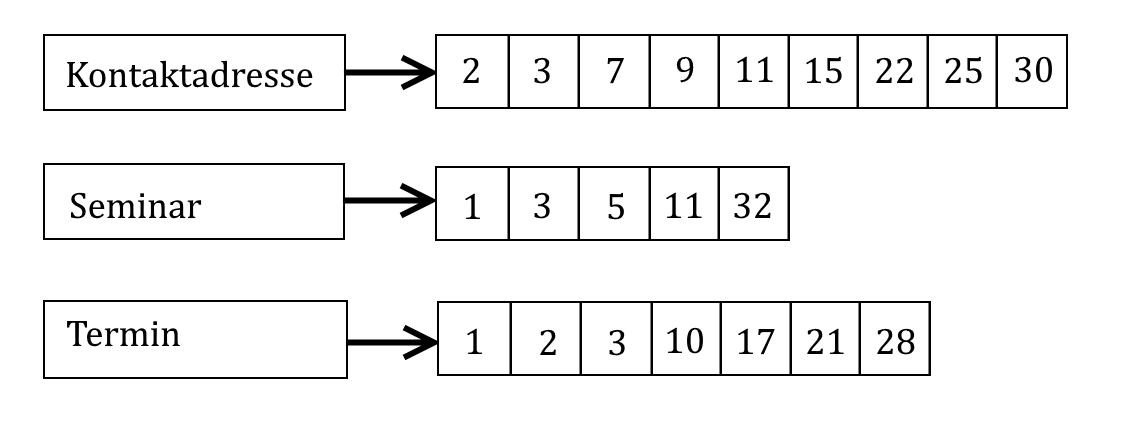
\includegraphics[width=1\textwidth]{images/inverted_list.png}
	\caption{Invertierte Listen zu Beispieltermen. Die Zahlen sind die Dokumentindizes, in denen der jeweilige Term vorkommt (Eigene Abbildung).}
	\label{abb1}
\end{figure}


%beispiel
\newpage
\subsubsection{Verarbeitung einer Anfrage}
Hier stellt sich die Frage, wie denn nun eine boolesche Anfrage, wie in Abschnitt \ref{formelzeugs} beschrieben, mithilfe invertierter Listen umgesetzt werden kann. \\
\paragraph{Elementare Anfrage}
Angenommen, es liegt eine elementare boolesche Anfrage in der Form $(t,t_1)$ vor. In der Praxis ist meist nach dem Vorkommen eines bestimmtes Wortes gefragt.\\
 Demnach entspricht das Attribut $t$ dem Term des gesuchten Wortes.\\ Da man auf dessen Vorkommen pr�ft, gelten f�r den Wertebereich $T = \{true, false\}$ und f�r den Attributwert $t_1 = true$. \\
 Die Verarbeitung einer solchen elementaren Anfrage geht relativ einfach: �ber den Index kann auf den Term schnell zugegriffen werden, vorausgesetzt dieser ist in der Sammlung enthalten. Trifft dies zu, kann einfach die gesamte zugeh�rige invertierte Liste als Resultat ausgegeben werden, da f�r alle enthaltenen Dokumente $t_1 = true$ gilt. \\
 \paragraph{AND-Verkn�pfungen}
 Wie sieht nun die Verarbeitung aus, wenn mehrere Anfragen miteinander verkn�pft werden? Hierzu wird zun�chst der AND - Operator betrachtet. Eine Anfrage liegt dann in der Form $(t,t_1)$ $AND$ $(s,s_1)$ vor, wie etwa bei dem Beispiel \textit{Kontaktadresse AND Seminar}, wobei gilt $t=Kontaktadress, t_1=true$ sowie $s=Seminar, s_1=true$.\\
Demnach werden alle Dokumente gesucht, in denen beide Terme auftauchen. Dazu wird der Durchschnitt aus den zugeh�rigen invertierten Listen gebildet. Betrachtet man die Abbildung \ref{abb1}, so ist der Durchschnitt f�r $D_{t,t_1} \cap D_{s,s_1} $ bzw. f�r $Kontaktadress \cap Seminar$ gleich der Ergebnisliste $\{3,11\}$. \\
\paragraph{OR-Verkn�pfungen}
Lautet die Anfrage hingegen $(t,t_1)$ $OR$ $(s,s_1)$ bzw. \textit{Kontaktadresse OR Seminar}, so sind alle Dokumente gesucht, in denen entweder $t_1$ oder $s_1$ oder auch beide Terme vorkommen. \\
Gesucht ist also die Vereinigung  $D_{t,t_1} \cup D_{s,s_1}$ bzw. $Kontaktadress \cup Seminar$. Dies ist die Vereinigung der invertierten Listen beider Terme. Im Falle des Beispiels \ref{abb1} lautet die Ergebnisliste f�r die Anfrage \textit{Kontaktadresse OR Seminar} $\{1,2,3,5,7,9,11,15,22,25,30,32\}$.\\
F�r beide Listenoperationen gilt, das die Indizes in den Ergebnislisten sortiert und Duplikate entfernt werden (\cite{Manning:08}, S.11).

\paragraph{Komplexe Ausdr�cke}
Wie werden komplex geschachtelte Ausdr�cke, die mehrere Operatoren enthalten, wie etwa $Kontaktadresse$ $AND$ $Seminar$ $AND$ $Termin$ verarbeitet?\\

Im Falle von mehreren $AND$-Operatoren ist es effizient, zun�chst die einzelnen invertierten Listen aufsteigend nach deren L�nge zu sortieren und dann von links nach rechts zu verarbeiten, indem das nachfolgende AND auf die Ergebnisliste des vorherigen Durchschnitts angewandt wird: \\
$(Seminar$ $AND$ $Termin)$ $AND$ $Kontaktadresse$ \\
Auf diese Weise werden die Listen, �ber die iteriert werden muss, m�glichst klein gehalten. Besitzt die kleinste Liste beispielsweise die L�nge eins, dann kann nach der ersten Iteration bereits abgebrochen werden, da zul�ssige L�sungen in allen drei Listen vorkommen m�ssen. \\

Bei mehreren $OR$-Operatoren werden die Ausdr�cke analog von links nach rechts verarbeitet, wobei die Sortierung nach L�nge hierbei keinen Vorteil bringt, da bei der $OR$-Operation ohnehin �ber alle Elemente iteriert werden muss. Die Verarbeitung w�rde demnach in der folgenden Reihenfolge erfolgen: \\
$(Kontaktadresse$ $OR$ $Seminar)$ $OR$ $Termin$




\chapter{Das Vektorraum-Modell}


\section{Funktionsprinzip}
\section{Term Frequency}
\section{Document Frequency}
\section{Inverted Document Frequency}
\section{$Tf \times idf$ Weighting}
\subsection{Formeln}

\section{\"Ahnlichkeitsfunktion}
\subsection{Euklidische Distanz}
\subsection{Cosine Similarity}
\subsection{Alternativen}

\chapter{Bewertung eines Information-Retrieval-Systems}
In diesem Kapitel wird erl�utert, wie sich Information-Retrieval-Systeme bewerten und vergleichen lassen. \\
 
Nachdem mit dem booleschen Retrieval und dem Vektorraummodell bereits zwei klassische Verfahren vorgestellt wurden, mit denen sich Information-Retrieval-Systeme realisieren lassen, liegt es nahe, nach einer Methode zum Bewerten und Vergleichen solcher Systeme zu suchen. 
Die Bewertungsmethode muss hierbei f�r verschiedenste Systeme geeignet sein, denn diese k�nnen sich in zahlreichen Punkten wie beispielsweise Dokumentformat, Dokumentrepr�sentation oder in der Art und Weise, wie Anfragen formuliert und Ergebnisse pr�sentiert werden, unterscheiden (\cite{Ferber:03}, S.84). \\

\section{Problem Relevanz}
Um ein Information-Retrieval-System hinsichtlich dessen Qualit�t beurteilen zu k�nnen, muss die Relevanz der zur�ckgelieferten Ergebnisse eingestuft werden.
Hiermit er�ffnet sich das Hauptproblem: Wann ist ein Dokument relevant? Allgemein formuliert l�sst sich dies so beantworten: Ein Dokument ist relevant, wenn es das in der Anfrage formulierte Informationsbed�rfnis des Nutzers befriedigt (\cite{Ferber:03}, S.85). 
Der Begriff l�sst sich zudem mathematisch wie in Definition \ref{Relevance} angegeben definieren (\cite{Ferber:03}, S.86). \\ 

\begin{definition}(Relevanz)\\
	\label{Relevance}
	Die Relevanz eines Dokuments f�r eine Anfrage ist eine Relation $r: D \times Q \rightarrow R$, wobei $D= \{D_1,...,d_m\}$ die Menge der Dokumente, $Q$ die Menge der Anfragen und $R$ eine Menge von Wahrheitswerten, im Allgemeinen die Menge $\{0,1\}$, ist. (Im Folgenden wird $R=\{0,1\}$ angenommen, wenn nichts anderes gesagt wird.)\\
	Die Relation $r$ wird im Allgemeinen durch Befragen von Experten zu konkreten Anfragen und Dokumentmengen ermittelt und als Tabelle oder in Form von Listen gespeichert. \\
\end{definition}

Da zum Bestimmen der Relation die Beurteilung von Experten erforderlich ist, l�sst diese Definition sofort erkennen, dass Relevanz stets von der subjektiven Wahrnehmung eines Anwenders abh�ngig ist: Jeder Nutzer entscheidet f�r sich selbst, ob er ein Dokument als relevant einstuft.

\section{Precision und Recall}
In diesem Abschnitt werden die beiden zur Bewertung notwendigen Evaluierungsma�e Precision und Recall vorgestellt.

\subsection{Precisison}
Precision bedeutet �bersetzt Pr�zision und bezeichnet den Anteil relevanter Dokumente an allen zur�ckgelieferten Dokumenten. Formel \ref{prec} beschreibt die Berechnung, wobei $\#$ die Kardinalit�t bezeichnet.

\begin{equation}
\label{prec}
Precision = \frac{\#(relevante \hspace{2mm} \textnormal{zur"uckgewonnene} \hspace{2mm} Dokumente)}{\#(\textnormal{zur"uckgewonnene} \hspace{2mm} Dokumente)}
\end{equation}


\subsection{Recall}
Recall kann mit Trefferquote �bersetzt werden und beschreibt die Frage, wie viele der relevanten Dokumente tats�chlich vom System zur�ckgeliefert wurden, was in Formel \ref{rec} gezeigt wird (\cite{Manning:08}, S.142-143). 

\begin{equation}
\label{rec}
Recall = \frac{\#(relevante \hspace{2mm} \textnormal{zur"uckgewonnene}  \hspace{2mm} Dokumente)}{\#(relevante \hspace{2mm} Dokumente)}
\end{equation}

\subsection{Veranschaulichung}
Die Bedeutung der Ma�e l�sst sich leichter anhand der Kontingenztafel \ref{tabelle} nachvollziehen. 
Kontingenztafeln sind H�ufigkeitstabellen und stammen aus der Statistik. Sie  beschreiben die gemeinsame Verteilung zweier Merkmale, in diesem Fall handelt es sich dabei um Relevanz und R�ckgewinnung (\cite{Engelhardt:14}). 

 \begin{table}
	\caption{Kontingenztafel (\cite{Manning:08}, S.143)}
	\begin{tabular}{l|l|l}
		\space & relevant & irrelevant \\
		\hline
		zur�ckgewonnen & true positives (tp) & false positives (fp) \\
		\hline
		nicht zur�ckgewonnen & false negatives (fn) & true negatives (tn)
	\end{tabular}
	\label{tabelle}
\end{table}

Das Precision-Evaluierungsma� l�sst sich anhand Tabelle \ref{tabelle} wie folgt beschreiben:

\begin{equation}
Precision = \frac{tp}{tp+fp}
\end{equation}

Pr�zision berechnet demnach, wie viele der als positiv eingestuften Ergebnisse, d.h. inklusive der \textit{false positives}, auch tats�chlich \textit{true postives}, d.h. relevante Resultate, sind.\\

Die Beschreibung f�r das Recall-Evaluierungsma� anhand Tabelle \ref{tabelle} lautet wie folgt:

\begin{equation}
Recall = \frac{tp}{tp+fn}
\end{equation}

F�r die Bestimmung des Recalls werden die \textit{true positives}, d.h. alle vom System korrekt als positiv eingestuften Ergebnisse, durch die Gesamtheit der relevanten Resultate dividiert. Wie sich aus der Tabelle entnehmen l�sst, sind dies die \textit{true positives} und die \textit{false negatives}, d.h. auch jene Dokumente, die f�lschlicherweise vom System als nicht relevant eingestuft wurden. Der Recall gibt deshalb kurz gesagt die Trefferquote an.



\section{Zwei Evaluierungsma�e}
Um ein System aussagekr�ftig bewerten zu k�nnen, reicht eines der beiden Ma�e nicht aus. 
Beispielsweise k�nnte ein System einen Recall von $100\%$ erreichen, indem es einfach alle Dokumente zur�ckliefert. 
Umgekehrt l�sst sich auch eine Precision von $100\%$ erzielen, wenn nur ein einziges Dokument gefunden wurde und dieses ein Treffer war. Vielleicht wurden hier allerdings eine ganze Reihe weiterer relevanter Dokumente nicht gefunden.
Deshalb werden stets beide Ma�e f�r eine qualitative Einsch�tzung eines Information-Retrieval-Systems ben�tigt.

\section{Durchf�hrung}
Eine Bewertung anhand der oben aufgef�hrten Evaluierungsma�e kann durchgef�hrt werden, wenn die folgenden Voraussetzungen gegeben sind (\cite{Manning:08}, S.140): \\

\begin{itemize}
	\item Vorgegebene Dokumentsammlung
	\item Feste Menge von Test-Anfragen
	\item Eine Relation $r$, die jedem Anfragen-Dokument Paar einen Wert $\in \{0,1\}$ f�r relevant bzw. irrelevant zuordnet
\end{itemize}
Leider sind f�r diese Arbeit jedoch die oben gelisteten Voraussetzungen nicht gegeben.
 Die Erzeugung einer repr�sentativen Test-Dokumentsammlung ist f�r die Problemstellung nicht m�glich, da die Art des Dokumentarchivs offen gehalten wurde. 
Selbst mit Beschr�nkung auf den Anwendungsfall E-Mails w�re in jedem Fall die zu erzeugende Anfragenmenge zu gro�, um sie im Rahmen dieser Arbeit bew�ltigen zu k�nnen, da Anfragen aus beliebigen W�rtern bestehen und zudem beliebig tief geschachtelt werden k�nnen. 
Aufgrund dieser Punkte musste auf eine Bewertung des Systems anhand von Precision und Recall verzichtet werden.
\chapter{Implementierung}

In diesem Kapitel wird beschrieben, auf welche Weise das System zur Informationssuche in einem Dokumentenarchiv basierend auf Textinhalt sowie Metadaten unter Verwendung der Programmiersprache Lisp realisiert wurde.

\section{Teilweise strukturierte Dokumente}
Besonderheit der Problemstellung ist das Vorliegen der Dokumente in semistrukturierter Form (siehe Abschnitt \ref{Problemstellung}). 
Dies erfordert das L�sen zweier Teilprobleme: Zum einen das Realisieren der Metadatensuche und zum anderen das Realisieren der Freitextsuche. Die Probleme wurden aufgrund der unterschiedlichen Anforderungen mit verschiedenen Verfahren gel�st. F�r die Metadatensuche wurde boolesches Retrieval verwendet, bei der Freitextsuche hingegen das Vektorraummodell.\\
Bevor erkl�rt wird, aus welchen Gr�nden diese Entscheidungen getroffen wurden, ist es wichtig, zun�chst eine Vorstellung zu haben, wie die zu durchsuchenden Dokumente des Archivs beschaffen sind. Hierzu zeigt Listing \ref{example} ein Beispiel. Beim Betrachten wird deutlich, dass jedes Dokument spezifische Eigenschaften besitzt, die jeweils durch einen Attributnamen und den zugeh�rigen Attributwert dargestellt sind. Beispielsweise ist \glqq datum\grqq{} ein Attributname und \glqq("Wed, 22 Jun 2017 07:47:51 +0200")\grqq{} der zugeh�rige Attributwert. Es k�nnen auch mehrere sehr �hnliche Attributnamen auftauchen, die sich lediglich durch Gro�- und Kleinschreibung unterscheiden, z.B. \glqq Betreff\grqq{} und \glqq BETREFF\grqq{}. Das System behandelt diese wie einen einzigen Attributnamen. \\
 Die Gesamtheit aller Attribute eines Dokuments bildet den Metadatenteil. Darauf folgt der unstrukturierte Freitextabschnitt.
 
\begin{lstlisting}[language=lisp, caption={Beispieldokument}
\label{example},
language=lisp]
;Metadaten

(absender ("<maximilianSchuster@mail.de>"))
(Betreff ("Umfrage"))
(datum ("Wed, 22 Jun 2017 07:47:51 +0200"))
(anzahlAnhaenge 0)
(Termin nil)

(ABSENDER-NAME "Maximilian Schuster")
(ABSENDER-MAIL-ADRESSE "maximilianSchuster@mail.de")
(EMPFAENGER ("John Schmitz"))
(EMPFAENGER-MAIL-ADRESSEN ("johnSchmitz@mail.de"))
(BETREFF "Umfrage")
(EMAIL-TYP "sent")
(QUELLBOXART "SENT")

;Freitext

Hallo John,

ich werde dir die Umfragenformulare schnellstm�glich per Post 
zukommen lassen.


Viele Gr��e
Maximilian Schuster

\end{lstlisting}

In der Regel enthalten die Dokumente weitaus mehr Attribute als in diesem Beispiel, zudem k�nnen sich die Attributwerte auch �ber mehrere Zeilen erstrecken. Zus�tzlich enthalten die Dokumente oft durch ein Semikolon gekennzeichnete Kommentare (siehe Listing \ref{example}, Z.1, Z.17), die vom System als Freitext interpretiert werden. \\
Beim gezeigten Beispiel handelt es sich zwar um eine E-Mail, es k�nnen allerdings auch andere Dokumente vorliegen. Die einzige Bedingung f�r die korrekte Funktionsweise des Systems ist, dass die im Archiv enthaltenen Dokumente die in Listing \ref{struct} vorgegebene Struktur erf�llen. Die Attribute k�nnen darum inhaltlich vollkommen abweichend ausfallen, abh�ngig davon welche Art von Archiv durchsucht wird.

\begin{lstlisting}[language=lisp, caption=Dokumentstruktur,label={struct},numbers=none]
(Attrubutename_1 Attributwert_1)
....
(Attributname_n Attributwert_n)

Freitext

\end{lstlisting}



\section{Initialisierungsschritte}
Beim Starten des Programms werden einige Initialisierungsschritte ausgef�hrt, die im folgenden Abschnitt beschrieben werden.

\subsection{Erstellen des Dokument-Dictionaries}
Zun�chst wird das Dokument-Dictionary angelegt. Dieses wird intern durch eine Hashtabelle realisiert, da dies in Lisp einem Dictionary\footnote{engl. W�rterbuch, bezeichnet assoziative Arrays, die aus Schl�ssel-Wert-Paaren bestehen (\cite{Nebel:13}, S.3)} am n�chsten kommt. \\
Eine Hashtabelle eignet sich ideal f�r schnelle Zugriffe und wurde aus diesem Grund gew�hlt. �ber eine Hashfunktion wird der Schl�ssel oder \textit{hash key} eines Elementes auf eine Position in der Tabelle abgebildet. Die Positionsberechnung anhand der Hashfunktion erfolgt schnell: Im Durchschnitt entspricht der Zugriff auf ein Element einem Index-Zugriff auf ein Feld, was in konstanter Laufzeit, d.h. in $O(1)$\footnote{Die O-Notation gibt die obere Komplexit�tsgrenze eines Algorithmus an (\cite{Esponda:12}, S.20).}, erfolgt. Erst, wenn Kollisionen auftreten, d.h. wenn mehrere Elemente auf dieselbe Position abgebildet werden und darum an dieser Stelle eine Liste von Elementen gespeichert ist, betr�gt die Laufzeit im schlimmsten Fall $O(n)$, wobei $n$ die L�nge der Liste bezeichnet (\cite{ITWissen:13}, \cite{Lux:14}, S.27). \\
  Zu jedem Dokument werden im Dokument-Dictionary die folgenden Punkte erfasst:
\begin{enumerate}
	\item \textit{docID}: Das Zuweisen einer einmaligen \textit{docID} in Form eines fortlaufenden Integer-Wertes, der den Sch�ssel des Dokuments darstellt.
	\item Dateipfad.
	\item Dokumentvektor (zu Beginn noch nicht initialisiert).
	\item Datum: Optionale Information, die zur verbesserten Ergebnisanzeige dient.
	\item Absender: ebenfalls optionale Information, die nur der Ergebnisanzeige dient.
\end{enumerate}

Dateipfad, Dokumentvektor, Datum und Absender werden in einem Struct zusammengefasst. Ein Struct ist eine Datenstruktur der Programmiersprache Lisp, die aus selbst definierten und mit Werten belegbaren Slots besteht und sich darum ideal eignet, um zusammengeh�rige Werte kompakt und schnell abrufbar zu speichern. Das Struct bildet den Wert oder \textit{hash value} des Dokuments. \\ 
Die  Punkte 4 und 5 k�nnen entfallen, da nicht alle Dokumente diese Metadaten beinhalten, insbesondere falls es sich nicht um E-Mails handelt. Das System wurde bewusst so flexibel wie m�glich gehalten, um auch andere Dateien verarbeiten zu k�nnen. Zur Veranschaulichung zeigt Abbildung \ref{docs} die Struktur eines Eintrags im Dokument-Dictionary.

\begin{figure} [http]
	
	\centering
	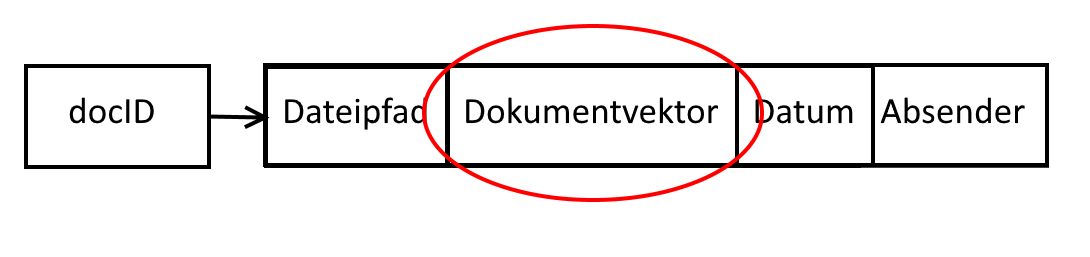
\includegraphics[width=1\textwidth]{images/docDict.png}
	\caption{Eintrag f�r ein Dokument im Dokument-Dictionary. Die Struct-Slots Datum und Absender k�nnen bei Fehlen dieser Metadaten leer bleiben. Im rot markierten Bereich wird sp�ter der Dokumentvektor eingetragen (eigene Abbildung).}
	\label{docs}
	
\end{figure}

\subsection{Verarbeiten der Dokumente}
Anschlie�end wird �ber alle Dokumente im Dokument-Dictionary iteriert, um die folgenden Schritte in der gezeigten Reihenfolge auszuf�hren:
\begin{enumerate}
	\item Aufteilen in Metadaten und Freitext.
	\item Verarbeiten der Metadaten.
	\item Verarbeiten des Freitextes.
\end{enumerate}



\subsubsection{Verarbeiten der Metadaten}
Die Metadaten werden zun�chst in Attributnamen und Attributwert zerlegt, um sie anschlie�end weiterverarbeiten zu k�nnen. 
F�r die Metadatensuche wurde boolesches Retrieval (siehe Kapitel \ref{bool}) eingesetzt, da eine klare Bedingung definiert werden kann: Der gesuchte Attributname muss im Dokument auftreten, d.h. jedes Dokument wird auf den Wertebereich $\{true, false\}$ abgebildet.
Allerdings muss zus�tzlich zum Auftreten noch gepr�ft werden, ob der Attributwert inhaltlich mit der Suchanfrage �bereinstimmt bzw. ob darin Teile der Anfrage auftauchen.\\
Um dies zu l�sen, wurde auf eine modifizierte Form der invertierten Liste (siehe Abschnitt \ref{inverted}) zur�ckgegriffen. Eine Term-Dokument Inzidenz Matrix wurde von vornherein aufgrund des zu hohen Speicherbedarfs ausgeschlossen. \\
Zum Verarbeiten der Metadaten wird eine Hashtabelle mit den Attributnamen als Schl�ssel erstellt, in der die folgenden Punkte, zusammengefasst in einem Struct, erfasst werden:

\begin{itemize}
	\item \textit{docID}: Eindeutiger Index des Dokuments, in dem das Attribut auftritt. Dieser geh�rt standardm��ig in die invertierte Liste.
	\item Typ: Dieser Eintrag gibt an, von welchem Datentyp der Attributwert ist, da dies �ber die Art der Suche darin entscheidet.
	\item Inhalt: Enth�lt den Attributwert. Dieser ist in der Regel so klein, dass er problemlos darin gespeichert werden kann und im Gegensatz zum Freitext keine weitere Verarbeitung erfordert. Durch das Unterlassen einer Indexierung der Attributwerte wird Speicher gespart.
\end{itemize}


Abbildung \ref{m} zeigt die modifizierte invertierte Liste anhand einiger Beispiel-Attribute. 
Hierbei ist zu beachten, dass beim Speichern der Attributnamen Gro�- und Kleinschreibung keine Rolle spielt, d.h. f�r die Keywords \glqq absender\grqq{} und \glqq ABSENDER\grqq{} wird nur ein einziger Schl�ssel angelegt. Mit dem Wort \glqq Keyword\grqq{} wird ausgedr�ckt, dass beide Begriffe sich auf ein und dasselbe Attribut beziehen. Kommen beide Keywords innerhalb eines Dokuments vor, gibt es unter dem entsprechenden Schl�ssel zwei Eintr�ge mit der gleichen \textit{docID}, aber unterschiedlichen Inhalten. Das Ignorieren von Gro�- und Kleinschreibung wird in dieser Implementierung im Allgemeinen angewendet, um W�rter, die sich nur hierin vom Suchbegriff unterscheiden, als �bereinstimmend zu erkennen. 

%MERGE!!!

\begin{figure} [http]
	
	\centering
	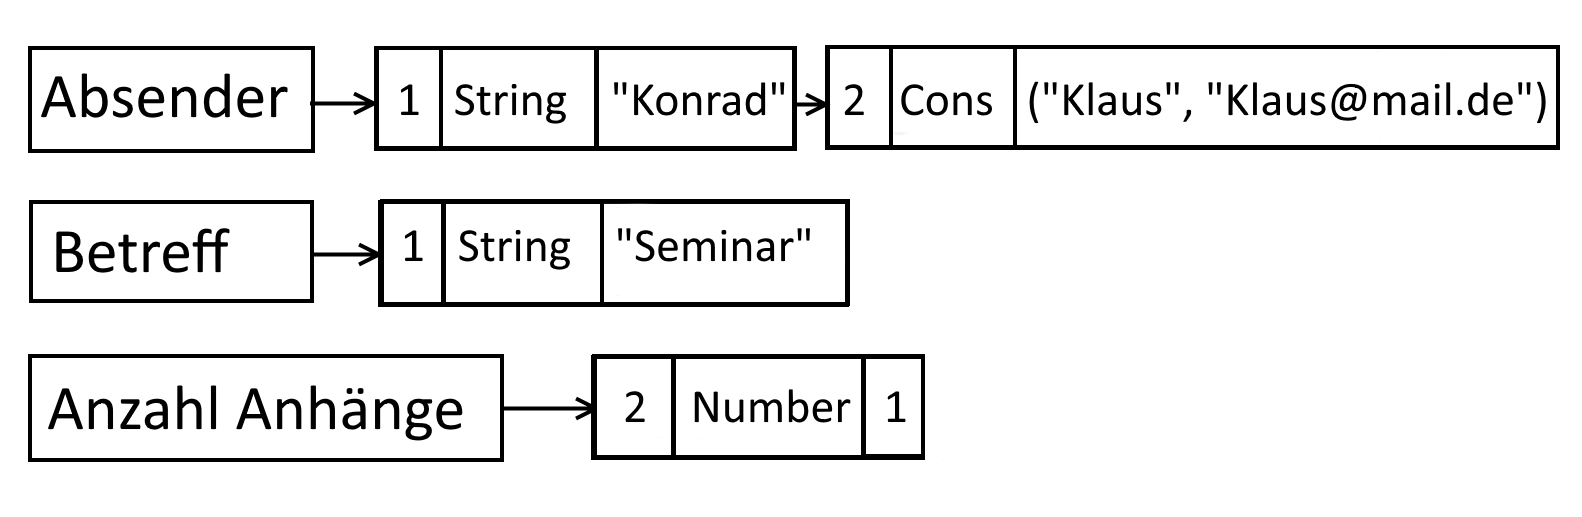
\includegraphics[width=1\textwidth]{images/mil.png}
	\caption{Modifizierte invertierte Liste zur Realisierung der Metadatensuche. Anstatt der \textit{docID}s werden Structs der Form (\textit{docID}, Typ, Inhalt) gespeichert (eigene Abbildung).}
	\label{m}
	
\end{figure}

\subsubsection{Verarbeiten des Freitextes}
F�r die Freitextsuche wurde das Vektorraummodell (siehe Kapitel \ref{vector}) gew�hlt, da dieses Teiltreffer sowie ein Ranking der Ergebnisse erm�glicht. Grundvoraussetzung f�r das Verfahren ist die Bestimmung des Vokabulars. Da jedes Dokument bereits in Metadaten und Freitext aufgeteilt wurde, liegen die Freitexte der Sammlung bereits isoliert vor. Es wird �ber diese Liste iteriert und pro Freitext werden jeweils die folgenden Schritte ausgef�hrt:
\begin{itemize}
	\item Zerlegung des Textes in Terme, wobei auf eine Lemmatisierung (siehe Abschnitt \ref{lemmatisierung}) verzichtet wurde, da dies den Rahmen der Arbeit sprengen w�rde. Zur zeilenweisen Zerlegung der Texte wurde das Package \textit{split-sequence} verwendet (\cite{Ionescu:16}).
	\item Zu jedem Term wird gepr�ft, ob dieser bereits im Vokabular enthalten ist. Falls nicht, wird er hinzugef�gt, vorausgesetzt es handelt sich nicht um ein deutsches oder englisches Stoppwort.
\end{itemize}

Stoppw�rter (siehe Abschnitt \ref{stop}) wurden aus dem Vokabular entfernt, um Speicherplatz zu sparen und die Suche zu beschleunigen, denn je kleiner die Dokument- und Anfragevektoren ausfallen, desto schneller erfolgt die Berechnung der �hnlichkeitswerte. Die englischen Stoppw�rter stammen aus \cite{webtools:13},  die deutsche Stoppwortliste aus \cite{Kohlfuerst:09}.

Nachdem das Vokabular vollst�ndig bestimmt wurde, werden die darin vorkommenden Terme indexiert. Hierf�r wird zun�chst ein Term-Dictionary angelegt, wobei auch hier die zugrunde liegende Datenstruktur eine Hashtabelle ist. Anschlie�end wird �ber das Vokabular iteriert und pro Term ein Eintrag in der Form (Index, $idf = 0$) angelegt. Der Index ist ein fortlaufender Integer-Wert, der den Term eindeutig identifiziert und dessen Position im Dokument- bzw. Anfragevektor bestimmt. Der idf-Wert muss erst noch ermittelt werden, darum wird er mit null initialisiert. Abbildung \ref{terms} zeigt den Aufbau eines Eintrags im Term-Dictionary.


\begin{figure} [http]
	
	\centering
	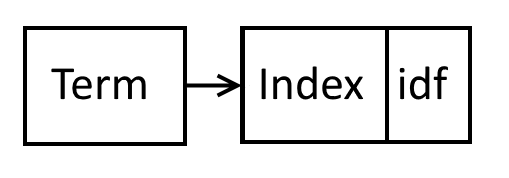
\includegraphics[width=0.5\textwidth]{images/termDict.png}
	\caption{Struktur f�r einen Eintrag im Term-Dictionary. Der Termname bildet den Schl�ssel, Index und $idf$ sind in einem Struct zusammengefasst. Der Index gibt die Position des Terms im Dokumentvektor an (eigene Abbildung).}
	\label{terms}
\end{figure}

Anschlie�end muss das Term-Dictionary mit idf-Werten gef�llt werden, weshalb �ber alle Freitexte iteriert wird und jeweils folgende Schritte ausgef�hrt werden:
\begin{itemize}
	\item Anlegen des Dokumentvektors in Form einer Hashtabelle, welche die Term-Indizes als Schl�ssel und deren noch zu bestimmende TF-IDF-Gewichte als Werte besitzt. 
	\item Taucht ein Term zum ersten Mal in der Sammlung auf, wird der zuvor mit null initialisierte $idf$-Slot im Term-Dictionary auf eins gesetzt.
	\item Kommt ein Term zum ersten Mal im Dokument vor und existiert bereits in der Sammlung, wird der $idf$-Wert um eins erh�ht.
	\item Beim ersten Auftauchen im Dokument wird der entsprechende Eintrag im Dokumentvektor auf die Termh�ufigkeit eins gesetzt. Die Position im Vektor wird durch den Termindex (gespeichert im Term-Dictionary) vorgegeben.
	\item F�r jedes erneute Vorkommen im Dokument wird die Termh�ufigkeit im Dokumentvektor um eins erh�ht.
	\item Ist der Freitext des aktuellen Dokuments vollst�ndig verarbeitet, kann der bereits angelegte Eintrag an der entsprechenden Stelle im Dokument-Dictionary (rot markiert in Abbildung \ref{docs}) mit dem hier erstellten Dokumentvektor initialisiert werden.
\end{itemize}

In den Dokumentvektoren werden nur Terme mit einem Gewicht gr��er null gespeichert. Fehlt ein Term in der Hashtabelle, so wird dies bei der Berechnung des Cosinus-Ma�es als Gewicht null interpretiert. Auf diese Weise wird Speicher gespart. \\
Noch enthalten die $idf$-Slots im Term-Dictionary die Dokumenth�ufigkeiten anstatt der $idf$-Werte.
Deshalb werden diese nach Formel \ref{idfb} in den $idf$-Wert umgerechnet. Es wurde sich f�r die Formel mit Logarithmus entschieden, um die Werte seltener Terme zu d�mpfen. 
Mit den $idf$-Werten k�nnen nun auch die TF-IDF-Gewichtungen bestimmt werden, weshalb die Termh�ufigkeiten in den Dokumentvektoren nach Formel \ref{tfidfc} umgerechnet werden. 
Anschlie�end k�nnen die Vektoren zur Verrechnung mit dem Anfragevektor verwendet werden. \\



\section{Suche}
Nachdem die Initialisierungsschritte ausgef�hrt wurden, kann der Nutzer die Suche starten. Er sieht auf der Benutzeroberfl�che, welche Attribute ihm als Suchbereiche zur Verf�gung stehen. Das Attribut \glqq Freitext\grqq{} ist hierbei immer vorhanden. 
Aufgrund der unterschiedlichen verwendeten Information-Retrieval-Verfahren werden Metadatensuche und Freitextsuche getrennt erkl�rt.

\subsection{Metadatensuche}
Die Metadatensuche verwendet boolesches Retrieval.
Lautet die Anfrage beispielsweise $Absender = Klaus$, wird auf die modifizierte invertierte Liste �ber den Schl�ssel $Absender$ zugegriffen. Anschlie�end wird �ber alle darin gespeicherten Structs iteriert, wobei zun�chst der Typ des Inhalts abgefragt wird, der �ber die Art der Suche entscheidet:
\begin{enumerate}
	\item \textbf{String}: Der Attributwert wird mit der vordefinierten Lisp-Funktion \textit{search} durchsucht. Die Suche ist erfolgreich, wenn die gesuchte Zeichenkette an einer beliebigen Stelle darin als Substring auftaucht.
	\item \textbf{Number}: Ist der Inhalt eine Zahl, wird die als String �bergebene Suchanfrage, wenn m�glich, zum Datentyp \glqq Number\grqq{} konvertiert. Hierbei sind auch als Wort ausgeschriebene Zahlen von null bis zw�lf konvertierbar. Ist kein Konvertieren m�glich, schl�gt die Suche fehl, da der Inhalt nicht zur Anfrage passen kann.
	\item \textbf{Liste}: Eine Liste entspricht in Lisp dem Datentyp \glqq Cons\grqq{} und wird rekursiv verarbeitet, um alle darin enthaltenen Elemente typspezifisch zu durchsuchen. Diese k�nnen Strings, Zahlen oder Listen sein.
\end{enumerate}
Liegt eine �bereinstimmung vor, wird die \textit{docID} des Dokuments der Ergebnisliste hinzugef�gt. 
Stellt der Nutzer die Anfrage f�r mehrere Attribute gleichzeitig, wird jedes ausgew�hlte Attribut nach dem Begriff durchsucht, d.h. es werden mehrere Metadatensuchen f�r die Anfrage ausgef�hrt.
Jedes Attribut besitzt seine eigene Ergebnisliste, sodass im Fall mehrerer Ergebnislisten diese gem�� booleschem Retrieval mit Mengenoperationen verrechnet werden: Ist $AND$ ausgew�hlt, wird aus den Listen der Durchschnitt gebildet, bei $OR$ die Vereinigung. Hierzu werden die vordefinierten Lisp-Funktionen \textit{intersection} und \textit{union} verwendet.\\
Nun liegt das finale Ergebnis f�r die Metadatensuche der Teilanfrage vor, es sei denn, der Nutzer hat $NOT$ ausgew�hlt, dann wird die Differenz zwischen den Dokumenten des Archivs und dem ermittelten Ergebnis zur�ckgegeben. Hierzu wurde die vordefinierte Funktion \textit{set-difference} verwendet.

\subsection{Freitextsuche}
\subsubsection{Erstellen des Query-Vektors}
Die Freitextsuche verwendet das Vektorraummodell, darum muss eine Anfrage erst in einen Vektor umgewandelt werden. Wie beim Dokumentvektor wird auch hier eine Hashtabelle als Datenstruktur verwendet. 
F�r jeden Term wird dessen Index im Term-Dictionary abgefragt. Vorausgesetzt, der Term existiert im Vokabular, wird dieser Index zum Schl�ssel und die Termh�ufigkeit in der Anfrage zum Wert. Ausnahme sind Stoppw�rter, die bei der Suche ignoriert werden. Der Nutzer erh�lt in diesem Fall eine Warnmeldung. Anschlie�end wird die Termh�ufigkeit mit dem $idf$-Wert multipliziert, sodass der Query-Vektor die finalen TF-IDF-Gewichtungen enth�lt.\\
Damit wird die Anfrage genau wie ein Dokument behandelt, mit dem einzigen Unterschied dass bestimmte Terme nicht im Vektor eingetragen und gewichtet werden, da sie im Archiv nicht vorkommen und darum f�r die Suche irrelevant sind.\\
Abbildung \ref{query} veranschaulicht das Erstellen des Query-Vektors anhand eines Beispiels.
\subsubsection{Finden der Resultate}
Zum Bestimmen der Suchergebnisse f�r die Freitextsuche wird �ber alle Dokumente iteriert, um folgende Schritte auszuf�hren:

\begin{itemize}
	\item Zugriff auf den Dokumentvektor.
	\item Berechnung des Cosinus-Ma�es (siehe Formel \ref{cos}) zur Bestimmung der �hnlichkeit zwischen Dokument- und Query-Vektor.
	\item Hinzuf�gen des �hnlichkeitswertes (Score) inklusive \textit{docID} zur Ergebnisliste. 
	\item Sortieren der Ergebnisliste anhand der erzielten Scores.
\end{itemize}

\begin{figure} [http]
	
	\centering
	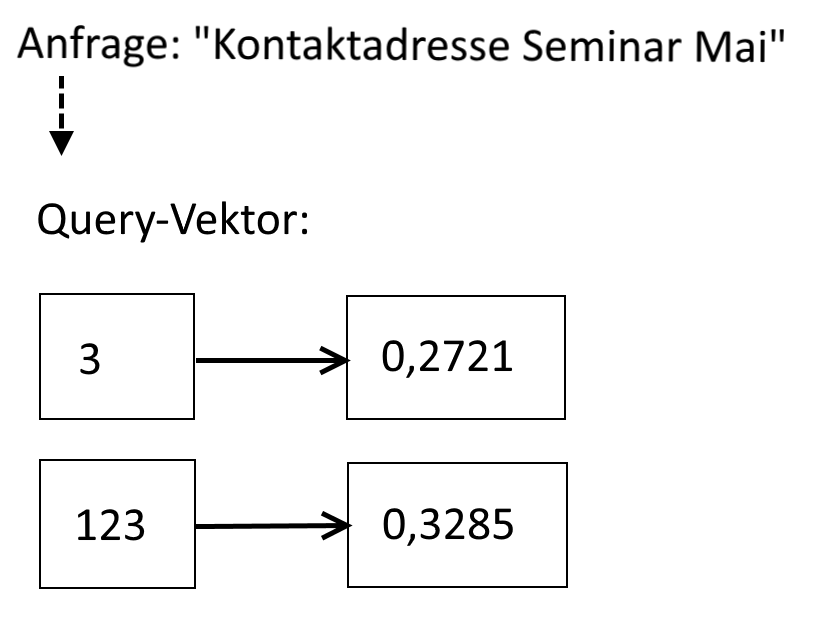
\includegraphics[width=0.5\textwidth]{images/Umwandlung.png}
	\caption{Umwandlung einer Anfrage in den entsprechenden Query-Vektor. \glqq Kontaktadresse\grqq{} besitzt den Index 3, \glqq Seminar\grqq{} den Index 123. Mai kommt im Archiv nicht vor, darum wird der Term ignoriert. Alle Indizes ungleich 3 und 123 sind als mit 0 gewichtet zu interpretieren (eigene Abbildung).}
	\label{query}
\end{figure}



\section{Verrechnung der Suchergebnisse}
Die Resultate beider Suchverfahren m�ssen miteinander kombiniert werden, wobei der Score ein Problem darstellt, da Metadaten-Resultate keinen besitzen. Gel�st wurde dies wie folgt:
\begin{itemize}
	\item Jedes Dokument in der Metadaten-Ergebnisliste erh�lt den Score eins.
	\item Ist $AND$ ausgew�hlt, wird der Durchschnitt der Ergebnislisten beider Suchverfahren gebildet und Metadaten-Score sowie Freitext-Score werden addiert.
	\item Ist $OR$ ausgew�hlt, wird die Vereinigung beider Suchen gebildet und Metadaten-Score sowie Freitext-Score der Dokumente, die in beiden Ergebnislisten vorkommen, werden addiert.
\end{itemize}
Da die Anfrage beliebig tief geschachtelt vorliegen kann, ist es m�glich, dass sich der Score eines Dokuments mit dem Stellen weiterer Teilanfragen erh�ht: 
Das Gesamtergebnis wird mit jeder neuen Teilanfrage auf dieselbe Weise wie soeben beschrieben verrechnet, d.h. je nach selektiertem Operator ($AND$ oder $OR$) wird der Durchschnitt oder die Vereinigung aus Gesamt- und Teilanfrage mit entsprechender Addition der Scores durchgef�hrt.
Demnach erh�lt ein Dokument, dass f�r f�nf Teilanfragen einen Treffer in der Metadatensuche liefert, den Score f�nf. Handelt es sich hingegen um einen nicht ganzzahligen Wert, z.B. $5.27$, kamen noch Treffer in der Freitextsuche hinzu. \\
Auf diese Weise kann der Nutzer in etwa absch�tzen, wie wichtig ein Dokument f�r seine Anfrage war und auf welche Weise das Ergebnis zustande kam, da ein nicht ganzzahliger Score nur durch eine erfolgreiche Freitextsuche entsteht.




\chapter{Die Benutzeroberfl\"ache}
Dieses Kapitel soll die Konzeption der Oberfl�che begr�nden und deren Nutzung erl�utern.\\

\section{Anforderungen}
Die Benutzeroberfl�che muss die folgenden, aus der Problemstellung resultierenden Funktionalit�ten erf�llen:
\begin{enumerate}
	\item W�hlen, Festlegen und �ndern des Suchverzeichnisses
	\item Ausw�hlen der Keywords
	\item Ausw�hlen der Freitextsuche
	\item Eingabe des Suchtextes
	\item Logische Operatoren zur externen Verkn�pfung zur Verf�gung stellen
	\item Logische Operatoren  zur internen Verkn�pfung zur Verf�gung stellen
	\item Anzeigen der Anfrage
	\item Starten der Suche
	\item Zur�cksetzen der Anfrage
	\item Anzeige der Resultate 

	
\end{enumerate}

Neben den oben genannten inhaltlichen Anforderungen sind noch weitere Punkte bez�glich Anwenderfreundlichkeit zu ber�cksichtigen: \\
\begin{enumerate}
\item �bersichtlichkeit
\item Intuitive Bedienbarkeit, d.h. der Nutzer soll m�glichst wenig nachdenken m�ssen
\end{enumerate}

Die Realisierung  der soeben beschriebenen Anforderungen wird in den folgenden Abschnitten erl�utert.

\section{Grundaufbau der Oberfl�che}
Die Oberfl�che wurde, um dem Nutzer eine gewisse �bersichtlichkeit zu bieten, in drei Bereiche gegliedert, die in Abbildung \ref{overview} gezeigt sind. \\
Der oberste Bereich beinhaltet die Verzeichnisauswahl, da dies der erste Schritt ist, der vom Anwender ausgef�hrt werden muss.\\
In der Mitte befindet sich die Anzeige der Gesamtanfrage, weil sie sich dort sofort im Blickfeld des Nutzers befindet. \\
Die Editierung der Teilanfragen wurde im unteren Teil der Oberfl�che untergebracht, weil sich hier die meisten Bedienungselemente befinden, weshalb jede andere Position unweigerlich Einbu�en  bez�glich �bersichtlichkeit zur Folge h�tte. \\
Funktional zusammengeh�rige Elemente wurden hierbei stets nah beieinander angeordnet, was dem Gesetz der N�he entspricht. \\
Dieses Gesetz besagt, dass Elemente, die nah zusammen liegen, vom Anwender als zusammengeh�rig wahrgenommen werden (\cite{Hofer:17}, S.17).
\begin{figure} [http]
	\centering
	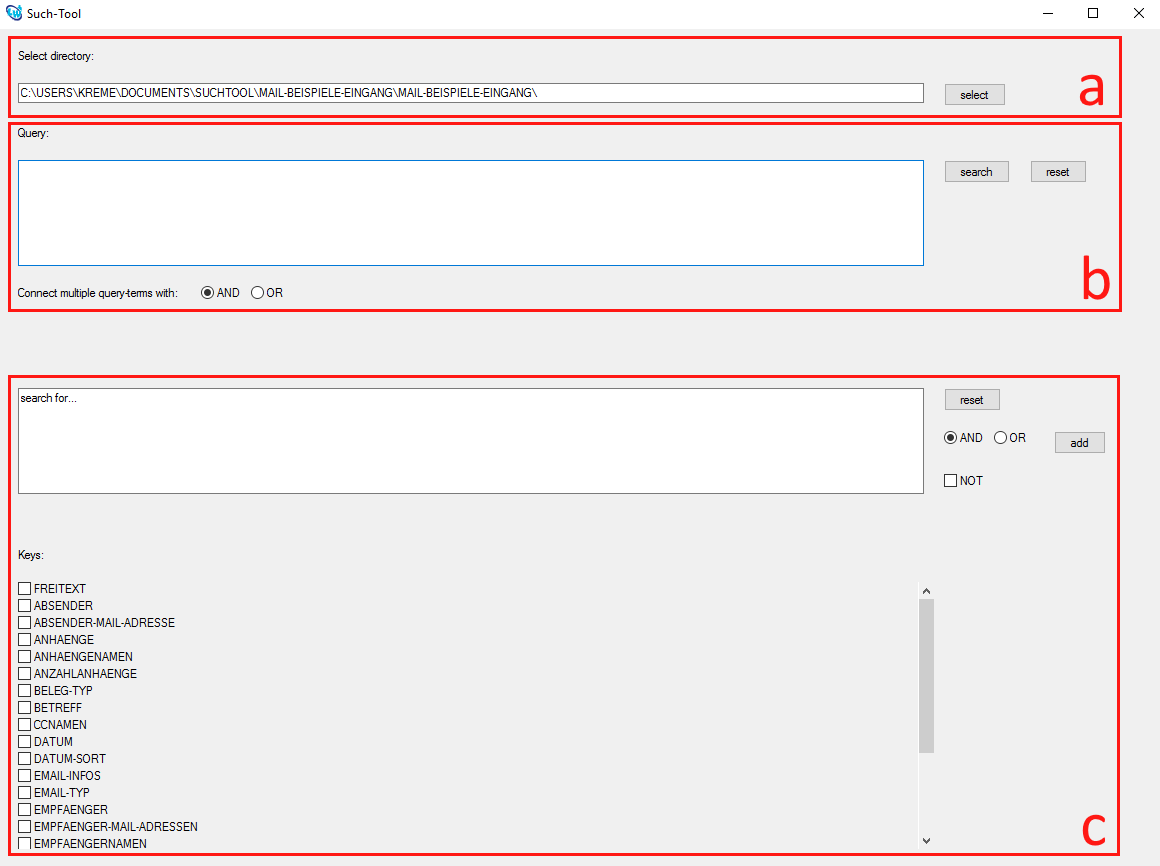
\includegraphics[width=1\textwidth]{images/overview.png}
	\caption{Gliederung der Benutzeroberfl�che. Teil \textit{a} beinhaltet die Verzeichnisauswahl, Teil \textit{b} die gesamte Suchanfrage und Teil\textit{c} die Eingabe der Teilanfrage (Eigene Abbildung).}
	\label{overview}
	
\end{figure}

\section{Verzeichnisauswahl}
Die Verzeichnisauswahl (siehe Abbildung \ref{overview} Teil a) besteht aus einem Textfeld und einem rechts daneben befindlichen Button mit der Aufschrift \glqq select\grqq{}, welcher das Auswahlmen� �ffnet.\\
Dieses wird in einem seperaten Pop-Up-Fenster angezeigt (siehe Abbildung \ref{select}) und besitzt zwei M�glichkeiten, ein Verzeichnis zu selektieren: \\
\begin{enumerate}
	\item Eintippen des Pfads in ein Textfeld
	\item Auswahl des Verzeichnisses �ber ein Dropdown-Men�
\end{enumerate}

Der Nutzer muss die Wahl mit \glqq ok\grqq{} best�tigen bzw. kann den Dialog �ber \glqq cancel\grqq{} abbrechen. \\
Anschlie�end wird der selektierte Verzeichnispfad im Textfeld angezeigt.

\begin{figure} [http]
	
	\centering
	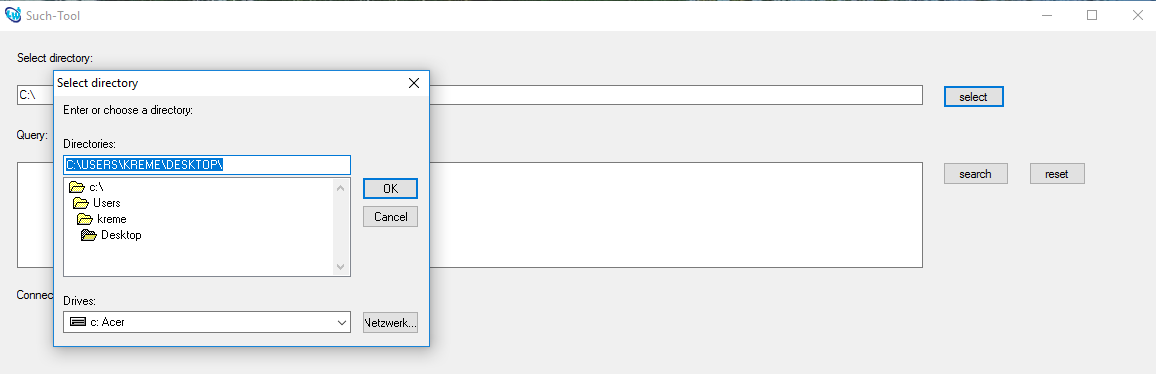
\includegraphics[width=1\textwidth]{images/Select.png}
	\caption{Verzeichnisauswahl (Eigene Abbildung)}
	\label{select}
	
\end{figure}

\section{Suchanfrage}
Im unteren Teil der Benutzeroberfl�che (siehe Abbildung \ref{overview} Teil c) befinden sich die Keywords. \\
Diese wurden als ausw�hlbare Checkboxen realisiert, welche sich auf einem vertikal scrollbaren Panel befinden. So ist sichergestellt, das eine beliebig gro�e Anzahl Keywords angezeigt werden kann. \\
Die Freitextsuche ist �ber die erste Checkbox \glqq Freitext\grqq{} ausw�hlbar, womit die Freitextsuche wie ein zus�tzliches Keyword behandelt wird, das sich in die Benutzeroberfl�che einf�gt. 
Dies ist gewollt, denn der Anwender soll nicht mitbekommen, dass das Suchen im Freitext intern anders implementiert ist als die �brigen Auswahlm�glichkeiten. \\

\subsection{Zusammenstellung der Teilanfrage}
Im Textdisplay wird die Anfrage vom Nutzer eingegeben und l�sst sich �ber \glqq reset\grqq{} bequem zur�cksetzen. \\
Die ausgew�hlten Checkboxen bestimmen dar�ber, in welchen Bereichen nach der Anfrage gesucht werden soll, wobei beliebig viele auf einmal selektierbar sind. \\
Im Falle mehrerer ausgew�hlter Bereiche lassen sich die Teilergebnisse mit $AND$ sowie $OR$ verkn�pfen. Beide M�glichkeiten lassen sich �ber zwei Radio-Buttons w�hlen, wobei $AND$ die Standardauswahl ist.\\
Zus�tzlich l�sst sich die Anfrage durch das Ausw�hlen der Checkbox $NOT$ negieren. Der Operator bezieht sich hierbei auf das Gesamtergebnis, wenn die Verkn�pfung bereits erfolgt ist. M�chte man Bereiche einzeln negieren, m�ssen die Anfragen getrennt eingegeben werden.\\
Das Dr�cken von \glqq Add\grqq{} f�gt die Teilanfrage der Gesamtanfrage hinzu. Sie wird dann auf dem Display im mittleren Bereich angezeigt (siehe Abbildung \ref{overview} Teil b).\\

\subsection{Beispiel}
Um die einzelnen Schritte besser nachvollziehen zu k�nnen, sei ein Beispiel anhand von Abbildungen gezeigt. \\
Abbildung \ref{a} zeigt, wie der Begriff \glqq Dr. Claus-Peter Wirth\grqq{} im Absender oder in der Absender-Mail-Adresse gesucht werden soll. Das Dr�cken von Add best�tigt die Teilanfrage und er�ffnet die M�glichkeit, eine weitere zu stellen.

\begin{figure} [http]
	
	\centering
	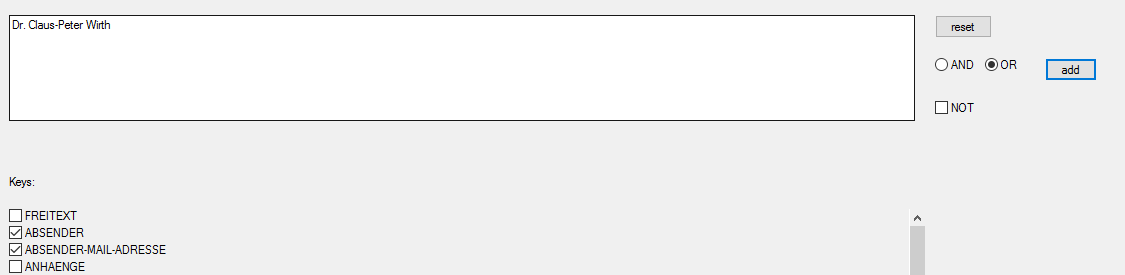
\includegraphics[width=1.1\textwidth]{images/a}
	\caption{Keywords ausw�hlen und intern verkn�pfen, hier OR (eigene Abbildung)}
	\label{a}
	
\end{figure}

Abbildung \ref{b} zeigt, wie der Begriff \glqq dfki\grqq{}\footnote{DFKI = Deutsches Forschungszentrum f�r K�nstliche Intelligenz} gesucht im Bereich Freitext gesucht werden soll. Es erfolgt erneutes Best�tigen durch \glqq Add\grqq{}.



\begin{figure} [http]
	
	\centering
	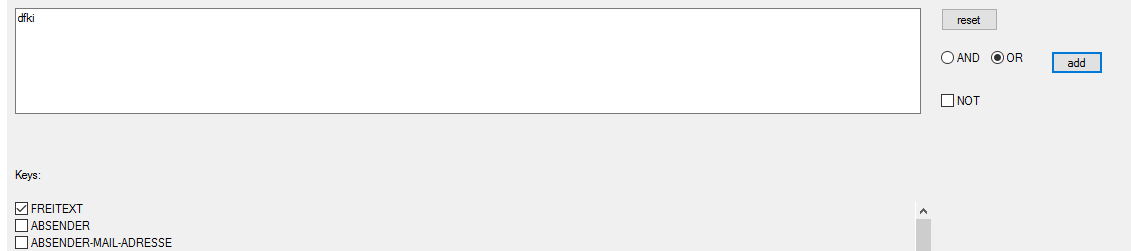
\includegraphics[width=1.1\textwidth]{images/b2}
	\caption{Freitextauswahl. Da nur ein Bereich ausgew�hlt ist, bleibt der selektierte $OR$-Operator ohne Wirkung (eigene Abbildung)}
	\label{b}
	
\end{figure}

\section{Gesamtanfrage}
Im vorigen Beispiel wurden zwei Teilanfragen gestellt, da zweimal Add  bet�tigt wurde.\\
 Das externe Verkn�pfen mehrerer Teilanfragen mit $AND$ bzw. $OR$ wird durch zwei Radio-Buttons unter dem oberen Textdisplay (siehe Abbildung \ref{overview}, Teil b) geregelt, wobei die Standardauswahl auch hier $AND$ ist. \\
Ist stattdessen $OR$ erw�nscht, muss diese Auswahl vor dem Bet�tigen des Add-Buttons getroffen worden sein, da eine �nderung des Operators im Nachhinein nicht mehr m�glich ist! \\
Abbildung \ref{c} zeigt, wie die im Display angezeigte Anfrage f�r das Beispiel mit dem Operator $AND$ aussieht. \\
In das obere Display l�sst sich vom Nutzer nichts eingeben, um die korrekte Anzeige der intern gespeicherten Anfrage zu gew�hrleisten. \\

\begin{figure} [http]
	
	\centering
	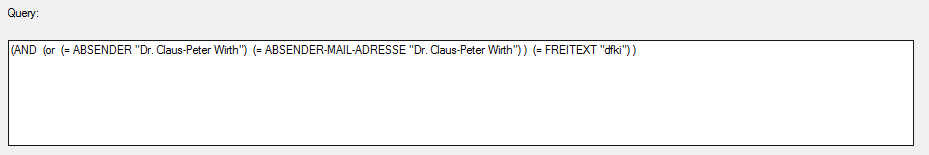
\includegraphics[width=1.1\textwidth]{images/b}
	\caption{Display (eigene Abbildung)}
	\label{c}
	
\end{figure}

\section{Ergebnis}
Der Nutzer kann die Gesamtanfrage mittels reset-Button komplett zur�cksetzen oder aber �ber den search-Button die Suche starten. \\
Das Dr�cken von \glqq search\grqq{} �ffnet ein Pop-Up-Fenster, welches die Resultate anzeigt und in Abbildung \ref{d} gezeigt ist. \\
In einer tabellarischen Ansicht werden die Rankposition, der Score, wenn m�glich Datum und Absender sowie der Dateipfad angezeigt. \\
Die Tabelle ist vertikal scrollbar (siehe Abbildung \ref{res}), falls viele Ergebnisse vorliegen. Eine Begrenzung wurde nicht vorgenommen, da keine Resultate ausgeschlossen werden sollen. Der Nutzer kann seine Wahl basierend auf der Ranking Position somit selbst treffen. \\
Die Eintr�ge der Tabelle lassen sich per Doppelklick ausw�hlen, sodass das zugeh�rige Verzeichnis mit der als ausgew�hlt markierten Datei bzw. die Datei selbst ge�ffnet wird. Welche dieser beiden Varianten gew�nscht ist, kann der Nutzer �ber die oben links angebrachten Radio-Buttons \glqq Open directory\grqq{} sowie \glqq Open file \grqq{} bestimmen. \\
Das Dr�cken von \glqq ok\grqq{} schlie�t das Ergebnis-Fenster.

\begin{figure} [http]
	
	\centering
	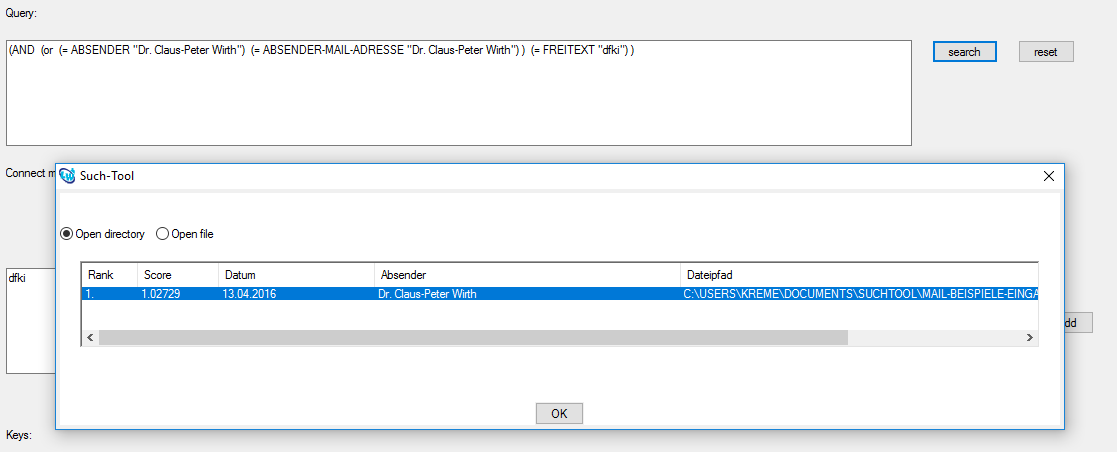
\includegraphics[width=1.1\textwidth]{images/c}
	\caption{Resultatfenster (eigene Abbildung)}
	\label{d}
	
\end{figure}

\begin{figure} [http]
	
	\centering
	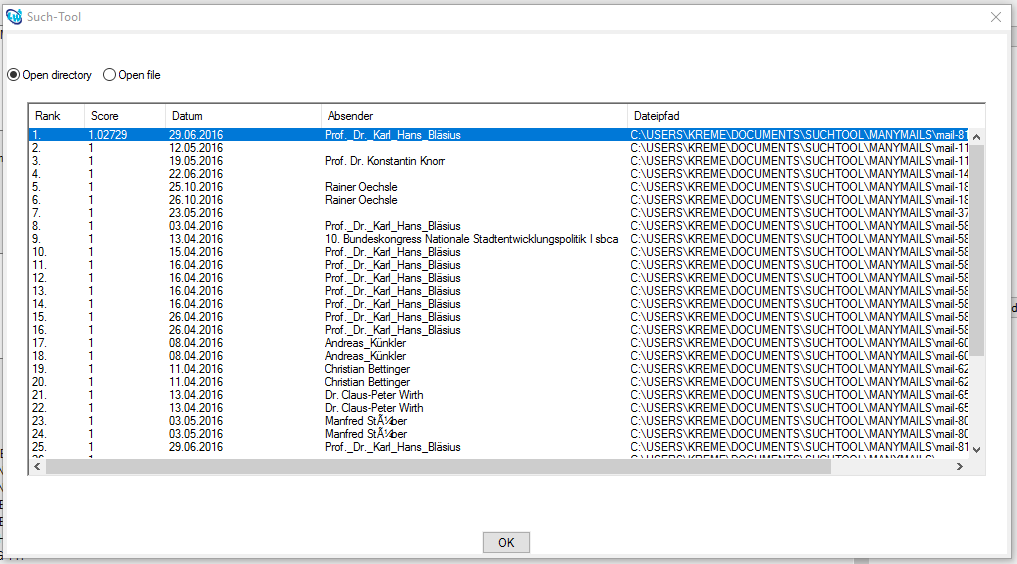
\includegraphics[width=1.1\textwidth]{images/results}
	\caption{Scrollbare Anzeige f�r viele Treffer (eigene Abbildung)}
	\label{res}
	
\end{figure}
\chapter{Zusammenfassung und Ausblick}

%In diesem Kapitel soll die Arbeit noch einmal kurz zusammengefasst werden. Insbesondere sollen die wesentlichen Ergebnisse Ihrer Arbeit herausgehoben werden. Erfahrungen, die z.B. Benutzer mit der Mensch-Maschine-Schnittstelle gemacht haben oder Ergebnisse von Leistungsmessungen sollen an dieser Stelle pr�sentiert werden. Sie k�nnen in diesem Kapitel auch die Ergebnisse oder das Arbeitsumfeld Ihrer Arbeit kritisch bewerten. W�nschenswerte Erweiterungen sollen als Hinweise auf weiterf�hrende Arbeiten erw�hnt werden.


\section{Zusammenfassung}

Im Kapitel Einleitung und Problemstellung wurde die Aufgabenstellung erl�utert, wobei sich bereits zeigte dass diese aufgrund des semistrukturierten Aufbaus der zu durchsuchenden Dokumente eine sehr spezifische L�sung erfordern w�rde. Die Unterteilung in Metadaten und Freitext sowie das logische Verkn�pfen der Suchbedingungen stellen die wesentlichen Herausforderungen dar.
Anschlie�end wurden die notwendigen theoretischen Kenntnisse vermittelt. Die Bedeutung des Begriffs Information Retrieval wurde erkl�rt und es zeigte sich, dass diese sehr weit gefasst ist,  weshalb diese Arbeit die ausgesprochen umfangreiche Thematik nur ansatzweise behandeln kann. Es wurden die beiden bekanntesten klassichen Information Retrieval  Verfahren vorgestellt; das boolesche Retrieval und das Vektorraummodell, sowie Methoden, anhand derer sich solche Modelle im Hinblick auf Qualit�t bewerten und Vergleichen lassen. Hierbei zeigte sich, dass eine solche Bewertung im Rahmen dieser Arbeit aufgrund des Aufwands leider nicht durchf�hrbar ist. \\
Im Implementierungskapitel wurde deutlich, dass die Verwendung eines der beiden klassischen Verfahren nicht ausreicht, die Kombination aus booleschen Retrieval und Vektorraummodell jedoch hervorragend passt. Das boolesche Retrieval musste allerdings geringf�gig modifiziert werden, indem nicht nur das Vorkommen der Attribute in den Dokumenten vermerkt wird, sondern auch deren Inhalt inklusive Datentyp. Beim Vektorraummodell zeigte sich, dass sich Speicher sparen l�sst, indem alle Elemente des Vektors, welche eine 0 enthalten, nicht eingetragen werden. \\
Zuletzt zeigte sich, dass die Benutzeroberfl�che eine nicht zu untersch�tzende Herausforderung darstellt,
da der Anwender sein Informationsbed�rfnis auf m�glichst unkomplizierte Art ausdr�cken k�nnen soll. Ein Information Retrieval System muss vom Nutzer auch verstanden werden. Es wurde sich daf�r entschieden, m�glichst einfache UI-Elemente wie CheckBoxes zu w�hlen sowie die Oberfl�che in drei thematische Bereiche zu gliedern, um die notwendige �bersicht zu bieten.




 \section{Ausblick: W�nschenswerte Erweiterungen}
Einige Erweiterungen konnten aus zeitlichen Gr�nden in der Implementierung nicht umgesetzt werden, sind jedoch w�nschenswert. \\
Die Im Kapitel Grundbegriffe beschriebene Lemmatisierung (siehe Abschnitt \ref{lemmatisierung}) w�rde eine gro�e Verbesserung hinsichtlich des Speicherbedarfs bedeuten, da weniger Terme gespeichert werden m�ssen. Zudem w�rde das Erg�nzen um Lemmatisierung auch die Suche verbessern, da auch Dokumente mit zum Suchbegriff verwandten W�rtern als Treffer gewertet werden. \\
Weiterhin w�nschenswert ist die Erg�nzung um Spelling Correction, d.h. um eine Rechtschreibkorrektur die �hnliche Suchbegriffe vorschl�gt, falls der Anwender sich bei der Eingabe vertippt hat. Dies w�rde die Anwenderfreundlichkeit des Systems erheblich steigern, insbesondere in F�llen in welchen der Anwender seinen Tippfehler nicht bemerkt und unerwartet keine Resultate erh�lt. Da Nutzer in der Regel Spelling Correction aus der allt�glichen Websuche gew�hnt sind, ist es w�nschenswert auch dieses Information Retrieval System damit auszustatten.


%-Stopwords \\
%-Lemmatisierung \\
%-Spelling Correction \\

% ...
%--------------------------------------------------------------------------
\backmatter                        		% Anhang
%-------------------------------------------------------------------------
\bibliographystyle{geralpha}			% Literaturverzeichnis
\bibliography{literatur}     			% BibTeX-File literatur.bib
%--------------------------------------------------------------------------
\printindex 							% Index (optional)
%--------------------------------------------------------------------------
\begin{appendix}						% Anh�nge sind i.d.R. optional
   %\chapter{Glossar}

\abbreviation{DisASTer}		{DisASTer (Distributed Algorithms Simulation Terrain), A platform for the Implementation of Distributed Algorithms}
\abbreviation{DSM}			{Distributed Shared Memory}
\abbreviation{AC}			{Linearisierbarkeit (atomic consistency)}
\abbreviation{SC}			{Sequentielle Konsistenz (sequential consistency)}
\abbreviation{WC}			{Schwache Konsistenz (weak consistency)}
\abbreviation{RC}			{Freigabekonsistenz (release consistency)}
			% Glossar   
   \chapter{Erkl�rung der Kandidatin / des Kandidaten}

\begin{description}[$\Box$~]
\item[$\Box$] Die Arbeit habe ich selbstst�ndig verfasst und keine anderen als die angegebenen Quellen- und Hilfsmittel verwendet.\\

\item[$\Box$] Die Arbeit wurde als Gruppenarbeit angefertigt. Meine eigene Leistung ist\\
...\\

Diesen Teil habe ich selbstst�ndig verfasst und keine anderen als die angegebenen Quellen und Hilfsmittel verwendet. \\

Namen der Mitverfasser: ...

\end{description}

\vspace{2cm}

\begin{minipage}[t]{3cm}
\rule{3cm}{0.5pt}
Datum
\end{minipage}
\hfill
\begin{minipage}[t]{9cm}
\rule{9cm}{0.5pt}
Unterschrift der Kandidatin / des Kandidaten
\end{minipage}	% Selbstst�ndigkeitserkl�rung
\end{appendix}

\end{document}
